%\chapter{Equations of Motion}
\chapter{运动方程}

由于地震形变的幅度小,使得建立完全线性化的地球自由振荡理论成为可能;本章我们来推导初始状态为静态平衡的地球模型的无穷小弹性-引力形变所满足的线性化运动方程和边界条件。我们将采用三种不同的方法:(1)对上一章中得出的严格的欧拉守恒定律和边界条件直接做系统的线性化;(2)对严格的拉格朗日守恒定律做类似的线性化;(3)将哈密顿原理应用于一个来自对动能加上弹性-引力能的收支做独立分析而得到的作用量。得到的结果将适用于具有任意给定密度和弹性结构的一般地球模型。这三种推导中主要的复杂因素是固态地壳与地幔中的初始偏应力,任何对横向密度不均匀地球模型的自洽处理都必须考虑这一点。这里的推导详细阐述并扩展了讨论一般地球模型形变的一些文章中的结果,特别是Dahlen (\citeyear{dahlen72};\citeyear{dahlen73}),\textcite{woodhouse&dahlen78},\textcite{valette86},和\textcite{vermeersen&vlaar91}。
%%%

%\section{Equilibrium Earth Model}
\section{平衡地球模型}
\index{Earth model!equilibrium|(}%
\index{equilibrium Earth model|(}%

%%%

%%%
我们假设地球是由许多液态和固态区域组成,这些区域由互不相交、光滑且封闭的界面隔开,这些界面被称为{\em 内部边界\/}。
\index{discontinuity!interior}%
\index{boundary!interior}%
\index{interior boundary}%
一些内部边界是密接的固-固边界,如莫霍洛维奇不连续面和上地幔相变面,另外一些则是无摩擦的固-液边界,如内核边界、核幔边界和海底。
\index{discontinuity!solid-solid}%
\index{boundary!solid-solid}%
\index{solid-solid boundary}%
我们用$\earth_{\rm S}$表示固态区域的集合,用$\earth_{\rm F}$表示液态区域的集合;用$\earth=\earth_{\rm S}\cup\earth_{\rm F}$表示模型的全部体积部分。所有内部固-固边界的集合由$\Sigma_{\rm SS}$表示,所有内部固-液边界的集合则由$\Sigma_{\rm FS}$表示。所有边界包含外表面$\p\earth$ 的集合,表示为$\Sigma=\p\earth\cup\Sigma_{\rm SS}\cup\Sigma_{\rm FS}$。
\index{boundary!exterior}%
\index{exterior boundary}%
我们仍然使用$\allspace$表示全空间,因而$\allspace -\earth$代表地球以外的空间。$\Sigma$的向外单位法向为$\bnh$,$\Sigma$的内外两侧分别为$-$侧和$+$侧。图~\ref{fig3.1}是一般地球模型横截面的示意图,其中标注了上述符号;不同区域的大小和形状不能按图示简单理解。我们在这里所阐述的理论也可以推广到更真实的有边界{\em 相交\/}的模型;
\index{boundary!intersecting}%
\index{intersecting boundary}%
然而,这会不必要地使变分和能量的分析复杂化。为简便起见,我们将主要关注在图中所示的“洋葱状”模型。
\begin{figure}[t]
\begin{center}
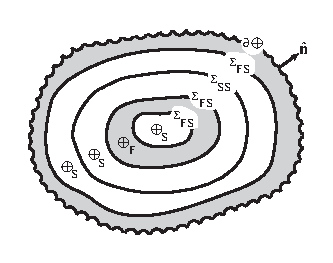
\includegraphics{../figures/chap03/fig01.eps}
\end{center}
\caption[Earth]{\label{fig3.1}
本书通篇使用的一般地球模型示意图以及各用来表示各区域和边界的符号。固态内核、地幔和地壳({\em 无阴影\/})构成$\earth_{\rm S}$,而液态外核和海洋({\em 阴影\/})构成$\earth_{\rm F}$ 。内部不连续面$\Sigma_{\rm FS}$和$\Sigma_{\rm SS}$以及自由表面$\partial\earth$的向外单位法向用$\hat{\bf n}$表示。要注意,所有的边界都假定为{\em 互不相交的\/};也不允许有封闭的固-液“海岸线”。}
\end{figure}
%%%

%%%

%%%
我们假定地球在地震发生之前处于力学平衡状态,相对于一组笛卡尔坐标轴$\bxh_1$, $\bxh_2$, $\bxh_3$静止不动,这组坐标轴绕着位于质心的原点$\bzero$以周日角速度$\bOmega$均匀自转。我们将$\earth$中或$\Sigma$上的点即物质质点用它们在该均匀转动参照系中的平衡位置$\bx$表示,而任何时候在使用角标符号时,所有的矢量和张量都是用它们在转动坐标系中的分量表示。我们在本章中引入与地球自转相关的科里奥利力和离心力,因为这样做并不会导致更多的复杂性。作为该地球模型考量的特例,得到的结果也适用于一个无自转($\bOmega=\bzero$)的地球。 
%%%

%%%

%%%
第二章中,我们发现区分欧拉梯度$\bdel_{\!\subr}$和拉格朗日梯度$\bdel_{\!\subx}$是有益的。
\index{gradient!Eulerian}%
\index{Eulerian gradient}%
\index{gradient!Lagrangian}%
\index{Lagrangian gradient}%
在初始构形中,$\bdel_{\!\subr}$和$\bdel_{\!\subx}$是相同的,而线性方程和边界条件仅需要相对于初始坐标的梯度$\bdel_{\!\subx}$;因而我们将从此略去下角标$\bx$,用简单的$\bdel$来表示$\bdel_{\!\subx}$。我们将用$d\/V$而不是用$d\/V^0$来做变形前体积元的符号,用$d\/\Sigma$而不是用$d\/\Sigma^0$来做变形前面积元的符号。边界$\Sigma$上的带方向的面元将简单地用$\bnh\,d\/\Sigma$表示,而不是前面所采用的$\bnh^0d\/\Sigma^0$。这些更改的目的只是为了避免在后面的公式中出现过多的上下角标。
%%%

%%%
令$\rho^0$为$\earth$内的初始密度分布,$\phi^0$为初始的引力势函数,以及
%%%
\eq
\label{3.gnotphinot}
\bg^0=-\bdel\phi^0
\en 
%%%

%%%
为相应的初始引力场。$\phi^0$和$\bg^0$这两个量可以用$\rho^0$写成
%%%
\eq
\label{3.phinot}
\phi^0=-G\int_{\subearth}\frac{\rho^{0\prime}}
{\|\bx-\bx'\|}\,dV'
\en
%%%

%%%
和
%%%
\eq
\bg^0=-G\int_{\subearth}\frac{\rho^{0\prime}\,(\bx-\bx')}
{\|\bx-\bx'\|^3}\,dV',
\en
%%%
%%%
这里撇号表示在积分变量$\bx'$处取值。假设密度$\rho^0$在地球以外为零;而$\phi^0$和$\bg^0$在$\allspace$内处处均不为零。在地球内部,势函数$\phi^0$满足泊松方程
%%%
\index{Poisson's equation}%
\eq
\label{3.Poisson0}
\nabla^2\phi^0=4\pi G\rho^0
\en
%%%

%%%
连同在边界$\earth$上的连续性条件
%%%
\eq
[\phi^0]^+_-=0,\qquad
[\bnh\cdot\bdel\phi^0]^+_-=0.
\en
%%%
在地球以外的$\allspace -\earth$区域,势函数是{\em 调和的}:$\nabla^2\phi^0=0$。
%%%
\index{harmonic potential}%
\index{potential!harmonic}%
\index{gravitational potential!harmonic}%

%%%
在变形前的构形中,柯西应力与两个Piola-Kirchhoff应力相同;我们用$\bT^0$表示地球模型内部的{\em 初始静应力\/}。
%%%
\index{initial static stress}%
\index{stress!initial}%
\index{stress!Cauchy}%
\index{Cauchy stress}%
\index{stress!first Piola-Kirchhoff}%
\index{stress!second Piola-Kirchhoff}%
\index{Piola-Kirchhoff stress!first}%
\index{Piola-Kirchhoff stress!second}%
%%%
在液态区域$\earth_{\rm F}$,必须有流体静力学初始应力:$\bT^0=-p^0\bI$,其中$p^0$是初始{\em 流体静力学压强}。
%%%
\index{pressure!hydrostatic}%
\index{hydrostatic pressure}%
\index{initial hydrostatic pressure}%
%%%
在固态区域$\earth_{\rm S}$,我们将压强$p^0$和初始{\em 偏应力\/}$\btau^0$定义为
%%%
\index{stress!deviatoric}%
\index{deviatoric stress}%
%%%
\eq
\label{3.taunotdef}
p^0=-\third\,{\rm tr}\,\bT^0,\qquad\btau^0=p^0\bI+\bT^0.
\en
%%%
%%%
式~(\ref{3.taunotdef})构成了初始应力的常规分解$\bT^0=-p^0\bI+\btau^0$,即分解为各向同性和偏向两部分;偏应力的迹为零:${\rm tr}\,\btau^0=0$。我们用$\varpi^0$表示边界$\Sigma$上牵引力的负法向分量
%%%
\eq
\label{3.pinotdef}
\varpi^0=-(\bnh\cdot\bT^0\cdot\bnh).
\en
%%%
在固-液边界$\Sigma_{\rm FS}$上,则有$\bnh\cdot\bT^0=-\varpi^0\bnh$,其中$\varpi^0$与液态一侧的初始压力$p^0$相等。
%%%

%%%
静态动量方程保证了均匀自转地球模型的力学平衡:
%%%
\index{static equilibrium}%
\index{equilibrium!static}%
\index{momentum equation!static}%
\eq
\label{3.eqcond2}
\bdel\cdot\bT^0=\rho^0\bdel(\phi^0+\psi),
\en
%%%
其中的离心势函数为
%%%
\eq
\label{3.centpot}
\psi=-\half[\Omega^2x^2-(\bOmega\cdot\bx)^2].
\en
%%%
\index{centrifugal potential}%
\index{potential!centrifugal}%
%%%
%%%
在液态区域$\earth_{\rm F}$,静态偏应力$\btau^0$为零,方程~(\ref{3.eqcond2})成为流体静力学平衡方程:
%%%
\index{hydrostatic equilibrium}%
\index{equilibrium!hydrostatic}%
\eq
\label{3.EQCOND}
\bdel p^0+\rho^0\bdel(\phi^0+\psi)=0.
\en
%%%
方程~(\ref{3.eqcond2})和~(\ref{3.EQCOND}) 必须在所有$\earth_{\rm S}$和$\earth_{\rm F}$区域内都要成立,且在边界$\Sigma$上需要满足牵引力连续性边界条件
%%%
\eq
\label{3.Tnotbc}
[\bnh\cdot\bT^0]^+_-=\bzero
\en
%%%
在地球的自由外表面$\p\earth$,牵引力必须为零:$\bnh\cdot\bT^0=\bzero$  
%%%
\index{Earth model!equilibrium|)}%
\index{equilibrium Earth model|)}%

\section{线性微扰}

%%%

%%%
我们采用运动的拉格朗日描述,将位置矢量$\br(\bx,t)$写为:
%%%
\eq
\label{3.dispdef}
\br(\bx,t)=\bx+\bs(\bx,t).
\en
其中$\bs$是质点$\bx$在$t$时刻偏离其平衡位置的{\em 位移\/}(见图~3.2)。
%%%
\index{displacement}%
\index{material particle}%
%%%
为了得到微小弹性-引力振荡所满足的线性化的运动方程和边界条件,我们将$\bs$视为一个小量,且系统性地忽略所有的阶数为$\|\bs\|^2$的项。在对质量和动量守恒定律做线性化之前,我们先讨论一些一般性的认识。为后续讨论方便起见,我们将地球以外$\allspace - \earth$区域的$\bs$定义为零。
%%%

\begin{figure}[!t]
\centering
\begin{tabular}{lr}
\begin{tabular}{l}
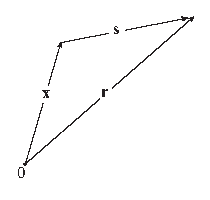
\includegraphics{../figures/chap03/fig02.eps}
\end{tabular}
&
\hspace{0.5cm}
\parbox{5.5cm}{\small
\vspace{0.05cm}
图~3.2.
%%%
%%%
初始位于点 $\bf x$ 的质点在$t$时刻移动到点${\bf r}({\bf x},t)={\bf x}+{\bf s}({\bf x},t)$。在本章所做的形变的线性化分析中,质点的{\em 位移\/}${\bf s}({\bf x},t)$均被认为是小量。
%%%
}
\end{tabular}
\end{figure}
\addtocounter{figure}{1}

\subsection{欧拉和拉格朗日微扰}
\index{perturbation!Eulerian|(}%
\index{Eulerian perturbation|(}%
\index{perturbation!Lagrangian|(}%
\index{Lagrangian perturbation|(}%
\index{q-stuff|(}%
\label{3.sec.perts}

%%%

%%%
对于任意的物理量$q$,我们定义一阶欧拉和拉格朗日微扰 $q^{\rm E1}$ 和 $q^{\rm L1}$ 为:
%%%
\eq
\label{3.qE1def}
q^{\rm E}(\br,t)=q^0(\br)+q^{\rm E1}(\br,t),
\en
\eq
\label{3.qL1def}
q^{\rm L}(\bx,t)=q^0(\bx)+q^{\rm L1}(\bx,t),
\en
%%%
其中$q^0$表示零阶初始值。如果形变小到足以允许线性化,那么精确到 $\|\bs\|$ 的一阶,我们有
%%%
\eq
\label{3.qE1rx}
q^{\rm E1}(\br,t)=q^{\rm E1}(\bx,t),\qquad
q^{\rm L1}(\bx,t)=q^{\rm L1}(\br,t).
\en
%%%
(\ref{3.qE1rx})式表明将一阶微扰$q^{\rm E1}$和$q^{\rm L1}$看作是$\br$还是$\bx$的函数是无关紧要的。因而我们之后将把所有的零阶和一阶变量都视为初始位置$\bx$的函数;而得到的线性化方程的适用区域则是变形前的地球体积$\earth$。与这些方程一起,我们还要加上在变形前的内外边界 $\Sigma$ 上成立的线性化边界条件。
%%%

%%%
将式~(\ref{3.dispdef})
和~(\ref{3.qE1def})--(\ref{3.qL1def})代入~(\ref{2.ELq}),并忽略二阶项,我们得到拉格朗日$q^{\rm L1}$和欧拉微扰$q^{\rm E1}$之间的关系:
%%%
\eq
\label{3.qL1qE1rel}
q^{\rm L1}=q^{\rm E1}+\bs\cdot\bdel q^0.
\en
%%%
公式~(\ref{3.qL1qE1rel})实质上是物质导数公式
%%%
\index{derivative!material}%
\index{material derivative}%
%%%
$D_t=\p_t+\bu^{\rm E}\cdot\bdel_{\!\subr}$线性化的、积分的形式。其物理解释是相似的:一个固定在运动质点上的观察者所感受到的一阶变化$q^{\rm L1}$包含在空间中定点$\bx$处的变化$q^{\rm E1}$以及质点在初始的空间梯度$\bdel q^0$中的位移$\bs$而导致的变化$\bs\cdot\bdel q^0$。$q$量可以是任何具有非零静态值的物理变量,如密度、引力或应力。
%%%
\index{gradient!initial spatial}%
\index{initial spatial gradient}%

\index{perturbation!Eulerian|)}%
\index{Eulerian perturbation|)}%
\index{perturbation!Lagrangian|)}%
\index{Lagrangian perturbation|)}%
\index{q-stuff|)}%

\subsection{形变的线性分析}
\index{deformation!linearized|(}%
\index{linearized deformation|(}%


%%%
不考虑形变张量$\bF$的两点特性,
%%%
\index{tensor!deformation}%
\index{deformation tensor}%
%%%
我们将其写成
%%%
\eq
\label{3.Fgrads}
\bF=\bI+(\bdel\bs)^{\rm T},
\en
%%%
其中$\bI$是单位张量。对于无限小形变,为方便起见可以将$\bF$分解为对称和反对称部分:
%%%
\eq
\label{3.epsomdef}
\bF=\bI+\beps +\bomega,
\en
%%%
其中
%%%
\eq
\beps=\half[\bdel\bs + (\bdel\bs)^{\rm T}],\qquad
\bomega=-\half[\bdel\bs - (\bdel\bs)^{\rm T}].
\en
\index{tensor!strain}%
\index{strain tensor}%
\index{tensor!rotation}%
\index{rotation tensor}%
%%%
对称部分$\beps=\beps^{\rm T}$是{\em 无穷小应变张量},反对称部分$\bomega=-\bomega^{\rm T}$ 则是{\em 无穷小转动张量}。精确到 $\|\bs\|$ 的一阶,我们可以将~(\ref{3.epsomdef}) 改写为另一种形式
%%%
\eq
\label{3.poldecomp}
\bF=(\bI+\bomega)\cdot(\bI+\beps)=(\bI+\beps)\cdot(\bI+\bomega).
\en
\index{polar decomposition}%
%%%
(\ref{3.poldecomp})可以被解释为小形变版的{\em 球极分解定理}~(\ref{2.poldecomp})。精确到 $\|\bs\|$ 的一阶,转动张量 $\bQ$ 以及右伸展和左伸展张量 $\bR$ 和 $\bL$ 由下式给定
%%%
\eq
\label{3.Qdef}
\bQ=\bI+\bomega,\qquad
\bR=\bL=\bI+\beps.
\en
%%%
精确到 $\|\bs\|$ 的一阶,$\bomega$的反对称性确保$\bQ$是正交的:
%%%
\eq
(\bI+\bomega)^{\rm T}\cdot(\bI+\bomega)=(\bI+\bomega)\cdot(\bI+\bomega)^{\rm T}=\bI.
\en
%%%
从公式~(\ref{2.EFrel})~或~(\ref{2.RErel}),我们可以看到,精确到 $\|\bs\|$ 的一阶,拉格朗日应变张量 $\bE^{\rm L}$ 成为
%%%
\index{tensor!strain}%
\index{strain tensor}%
\eq
\label{3.ELdef}
\bE^{\rm L}=\beps.
\en
%%%
鉴于~(\ref{3.poldecomp})--(\ref{3.ELdef})中的结果,我们此后一般会去掉“无穷小”这一形容词,而直接将$\beps$和$\bomega$称为应变张量和转动张量。
%%%

\index{tensor!strain-rate}%
\index{strain-rate tensor}%
\index{tensor!vorticity}%
\index{vorticity tensor}%
\index{tensor!rotation-rate}%
\index{rotation-rate tensor}%
%%%
将公式~(\ref{2.FrelG2})和~(\ref{2.GDW}) 线性化,我们获得精确到 $\|\bs\|$ 的一阶的欧拉应变率张量$\bD^{\rm E}$和转动率张量$\bW^{\rm E}$:
%%%
\eq
\label{3.DEdef}
\bD^{\rm E}=\p_t\beps,\qquad
\bW^{\rm E}=\p_t\bomega,
\en
\iffalse
i.e., they are are simply the time derivatives of the strain and
rotation tensors.
The first-order Eulerian velocity $\bu^{\rm E}$ is likewise simply
the time derivative of the displacement:
\fi
%%%
亦即它们只是应变张量和转动张量对时间的导数。同样地,一阶欧拉速度张量 $\bu^{\rm E}$ 是位移对时间的导数:
%%%
\eq
\bu^{\rm E}=\p_t\bs.
\label{3.uEdef}
\en
%%%
鉴于~(\ref{3.DEdef})--(\ref{3.uEdef})式,人们有时会认为对于无穷小形变,不需要区分欧拉和拉格朗日表述。然而,正如我们在~\ref{3.sec.perts}节看到的,这一结论对于像密度、引力和应力等具有零阶初值的变量并不成立。
%%%
\index{deformation!linearized|)}%
\index{linearized deformation|)}%

\subsection{体积和面积微扰}
\index{volume change|(}%
\index{area change|(}%

%%%
精确到 $\|\bs\|$ 的一阶,联系变形前后相应体积元的雅可比 $J={\rm det}\,\bF$ 可写为
%%%
\eq
\label{3.Jdef}
J=1+{\rm tr}\,\beps=1+\bdel\cdot\bs.
\en
%%%
在同阶近似下,形变张量 $\bF^{-1}$ 的逆可写为
%%%
\eq
\label{3.Finvdef}
\bF^{-1}=\bI-(\bdel\bs)^{\rm T}.
\en
%%%
将式~(\ref{3.Jdef})~和~(\ref{3.Finvdef})~代入~(\ref{2.ndsigrel}),并忽略二阶项,我们得到变形后面元$\bnh^td\/\Sigma^t$与相应的变形前的面元$\bnh\,d\/\Sigma$之间的线性化关系:
%%%
\eq
\label{3.ndsigrel}
\bnh^td\/\Sigma^t=(1+\bdel\cdot\bs)\,\bnh\,d\/\Sigma
-(\bdel\bs)\cdot\bnh\,d\/\Sigma.
\en
\index{gradient!surface}%
\index{surface gradient}%
%%%
涉及法向导数$\p_n\bs$的项会被消去,因此该结果可以仅用{\em 表面梯度\/} $\bdel^{\Sigma}=\bdel-\bnh
\hspace{0.2 mm}\p_n$改写为:
%%%
\eq
\label{3.ndsigrel2}
\bnh^td\/\Sigma^t=(1+\bdel^{\Sigma}\cdot\bs)\,\bnh\,d\/\Sigma
-(\bdel^{\Sigma}\bs)\cdot\bnh\,d\/\Sigma.
\en
%%%
(\ref{3.ndsigrel2})式中的第一项表示无穷小面元的面积变化,而第二项表示单位法向的偏转。精确到 $\|\bs\|$ 的一阶,这两个变化可以分别表示为:
%%%
\eq
\label{3.dsigrel}
d\/\Sigma^t=(1+\bdel^{\Sigma}\cdot\bs)\,d\/\Sigma,
\en
\eq
\label{3.nhatrel}
\bnh^t=\bnh-(\bdel^{\Sigma}\bs)\cdot\bnh.
\en
%%%
公式~(\ref{3.dsigrel})是体积关系~(\ref{3.Jdef})的面积形式;变形后与变形前体积元$d\/V^t$和$d\/V$的关系为:
%%%
\eq
d\/V^t=(1+\bdel\cdot\bs)\,d\/V.
\en
%%%
表示单位法向偏转的(\ref{3.nhatrel})式也可以用初等几何方法得到;(\ref{3.dsigrel})--(\ref{3.nhatrel})这两个关系式合起来意味着~(\ref{3.ndsigrel2})的结果。
%%%
\index{volume change|)}%
\index{area change|)}%

\subsection{应力微扰}
\index{stress!perturbations in|(}%

%%%
欧拉和拉格朗日柯西应力的一阶微扰的定义为:
%%%
\index{stress!Cauchy}%
\index{Cauchy stress}%
\eq
\label{3.TE1def}
\bT^{\rm E}=\bT^0+\bT^{\rm E1},\qquad
\bT^{\rm L}=\bT^0+\bT^{\rm L1}.
\en
%%%
固定在运动质点上的观察者所感受到的拉格朗日微扰$\bT^{\rm L1}$与空间中某一定点的欧拉微扰$\bT^{\rm E1}$可由(\ref{3.qL1qE1rel})式联系起来:
%%%
\eq
\label{3.TL1TE1rel}
\bT^{\rm L1}=\bT^{\rm E1}+\bs\cdot\bdel\bT^0.
\en
%%%
我们将第一类和第二类Piola-Kirchhoff应力增量分别用$\bT^{\rm PK1}$和$\bT^{\rm SK1}$表示。这些量以类似于~(\ref{3.TE1def})的方式定义为
%%%
\index{stress!first Piola-Kirchhoff}%
\index{stress!second Piola-Kirchhoff}%
\index{Piola-Kirchhoff stress!first}%
\index{Piola-Kirchhoff stress!second}%
\eq
\label{3.TPK1def}
\bT^{\rm PK}=\bT^0+\bT^{\rm PK1},\qquad
\bT^{\rm SK}=\bT^0+\bT^{\rm SK1}.
\en
%%%
将~(\ref{3.Jdef})--(\ref{3.Finvdef})、(\ref{3.TE1def})和~(\ref{3.TPK1def})代入~(\ref{2.tpkt1})和~(\ref{2.tskt1}),我们得到将Piola-Kirchhoff微扰$\bT^{\rm PK1}$和$\bT^{\rm SK1}$与拉格朗日柯西应力增量$\bT^{\rm L1}$相关联的线性化方程:
%%%
\eq
\label{3.TPK1TL1}
\bT^{\rm PK1}=\bT^{\rm L1}+\bT^0(\bdel\cdot\bs)
-(\bdel\bs)^{\rm T}\cdot\bT^0,
\en
\eq
\label{3.TSK1TL1}
\bT^{\rm SK1}=\bT^{\rm L1}+\bT^0(\bdel\cdot\bs)
-(\bdel\bs)^{\rm T}\cdot\bT^0-\bT^0\cdot\bdel\bs.
\en
%%%
相应的$\bT^{\rm PK1}$与$\bT^{\rm SK1}$之间的一阶关系可以通过线性化~(\ref{2.TPKrelTSK})或比较~(\ref{3.TPK1TL1})~和~(\ref{3.TSK1TL1})得到:
%%%
\eq
\label{3.TPK1TSK1}
\bT^{\rm PK1}=\bT^{\rm SK1}+\bT^0\cdot\bdel\bs.
\en
%%%
值得注意的是,$\bT^{\rm E1}$、$\bT^{\rm L1}$和$\bT^{\rm SK1}$均为对称的,而第一类Piola-Kirchhoff应力增量$\bT^{\rm PK1}$则不是;事实上,
%%%
\index{stress!first Piola-Kirchhoff!asymmetry of}%
\index{Piola-Kirchhoff stress!first!asymmetry of}%
\eq
\label{3.TPK1tr}
(\bT^{\rm PK1})^{\rm T}=\bT^{\rm PK1}
-\bT^0\cdot\bdel\bs+(\bdel\bs)^{\rm T}\cdot\bT^0.
\en
%%%
由~(\ref{3.TPK1TL1})而得到的~(\ref{3.TPK1tr})是~(\ref{2.TPKtr})式的线性化形式。在第~\ref{3.sec.constrel}节中,我们将讨论线性弹性本构关系,并将应力微扰$\bT^{\rm L1}$、$\bT^{\rm PK1}$和$\bT^{\rm SK1}$用位移梯度$\bdel\bs$来表示。
%%%
\index{stress!perturbations in|)}%

\subsection{引力微扰}
\index{gravitational perturbation|(}%
\index{perturbation!gravitational|(}%

%%%
引力势函数与引力场的欧拉和拉格朗日微扰分别定义为
%%%
\eq
\label{3.phiE1def}
\phi^{\rm E}=\phi^0+\phi^{\rm E1},\qquad
\bg^{\rm E}=\bg^0+\bg^{\rm E1},
\en
%%%
和
%%%
\eq
\label{3.phiL1def}
\phi^{\rm L}=\phi^0+\phi^{\rm L1},\qquad
\bg^{\rm L}=\bg^0+\bg^{\rm L1},
\en
%%%
这些微扰满足常用的一阶关系:
%%%
\eq
\label{3.phiEL1}
\phi^{\rm L1}=\phi^{\rm E1}+\bs\cdot\bdel\phi^0,\qquad
\bg^{\rm L1}=\bg^{\rm E1}+\bs\cdot\bdel\bg^0.
\en
%%%
可以将欧拉场微扰$\bg^{\rm E1}$写为相应的势函数微扰的梯度:
%%%
\eq
\label{3.gE1phiE1}
\bg^{\rm E1}=-\bdel\phi^{\rm E1}.
\en
%%%
$\bg^{\rm L1}$的相应结果更为复杂;从~(\ref{3.phiEL1})--(\ref{3.gE1phiE1})可见
%%%
\eq
\label{3.gL1phiL1}
\bg^{\rm L1}=-\bdel\phi^{\rm E1}-\bs\cdot\bdel\bdel\phi^0
=-\bdel\phi^{\rm L1}+\bdel\bs\cdot\bdel\phi^0.
\en
%%%
(\ref{3.gE1phiE1})~和~(\ref{3.gL1phiL1})~这两个关系之间的差异反映了经典引力势理论的固有的欧拉属性。在第~\ref{3.sec.grav}节中,我们将推导引力微扰$\phi^{\rm E1}$、$\bg^{\rm E1}$ 、$\phi^{\rm L1}$和$\bg^{\rm L1}$与位移$\bs$之间的线性积分关系。
%%%
\index{gravitational perturbation|)}%
\index{perturbation!gravitational|)}%

\section{线性化的守恒定律}
\index{conservation law!linearized|(}%

%%%
质量与动量守恒定律的线性化形式很容易得到。线性理论的一个固有特征是,在所有的能量分析中都要求二阶精度;因此,对能量守恒定律进行线性化处理是不够的。在第3.8节和3.9节中,我们将对弹性-引力能做一致性的二阶处理。
%%%
 
\subsection{线性化的连续性方程}
\index{conservation!of mass!linearized|(}%
\index{mass!conservation of!linearized|(}%

%%%
密度的欧拉和拉格朗日微扰$\rho^{\rm E1}$和$\rho^{\rm L1}$定义为
%%%
\eq
\label{3.rhoE1def}
\rho^{\rm E}=\rho^0+\rho^{\rm E1},\qquad
\rho^{\rm L}=\rho^0+\rho^{\rm L1}.
\en
%%%
通过线性化欧拉和拉格朗日质量守恒定律,可以将这两个微扰与位移$\bs$联系起来。将~(\ref{3.rhoE1def})的分解式代入欧拉连续性方程~(\ref{2.cont}),并对时间积分,精确到 $\|\bs\|$ 的一阶,我们得到
%%%
\eq
\label{3.contE}
\rho^{\rm E1}=-\bdel\cdot(\rho^0\bs),
\en
\index{continuity equation}%
%%%
将~(\ref{3.Jdef})和~(\ref{3.rhoE1def})一起代入拉格朗日质量守恒方程~(\ref{2.lagmass})可得(精确到相同量级):
%%%
\eq
\label{3.contL}
\rho^{\rm L1}=-\rho^0(\bdel\cdot\bs),
\en
%%%
我们放心的看到,(\ref{3.contE})和(\ref{3.contL})这两个微扰有下面的关系:
%%%
\eq
\rho^{\rm L1}=\rho^{\rm E1}+\bs\cdot\bdel\rho^0,
\en
%%%
它与普遍的关系式~(\ref{3.qL1qE1rel})一致。
%%%

%%%
(\ref{3.contL})式为质点位移$\bdel\cdot\bs$的散度提供了物理解释。定义拉格朗日比容微扰$\tau^{\rm L1}$为
%%%
\eq
\tau^{\rm L}=\tau^0+\tau^{\rm L1},
\en
%%%
其中$\rho^0\tau^0=1$,我们看到
%%%
\eq
\label{3.divdef}
\bdel\cdot\bs=-\frac{\rho^{\rm L1}}{\rho^0}=\frac{\tau^{\rm L1}}{\tau^0}.
\en
\index{specific volume}%
\index{volume!specific}%
%%%
显然,$\bdel\cdot\bs$是质点$\bx$在$t$时刻单位质量的体积的相对变化。~(\ref{3.divdef})式可以看作是~(\ref{2.divdef})的线性化、积分的形式。
%%%
\index{conservation!of mass!linearized|)}%
\index{mass!conservation of!linearized|)}%

\subsection{线性的化动量方程}
\index{conservation!of momentum!linearized|(}%
\index{momentum!conservation of!linearized|(}%
\index{equations of motion|(}%

%%%
要得到欧拉动量方程的线性化形式,我们将表达式 ~(\ref{3.TE1def})、(\ref{3.phiE1def})和~(\ref{3.rhoE1def}))代入精确关系式~(\ref{2.finmomeqn})。忽略$\|\bs\|$的二阶项,并消去静态平衡条件~(\ref{3.eqcond2})式,可得:
%%%
\eq
\label{3.momeqn}
\rho^0(\p_t^2\bs+2\bOmega\times\p_t\bs)=\bdel\cdot\bT^{\rm E1}
-\rho^0\bdel\phi^{\rm E1}-\rho^{\rm E1}\bdel(\phi^0+\psi).
\en
%%%
严格来讲,这一结果适用于变形后地球内部的点$\br$,而不是在变形前地球内部的点$\bx$,且梯度为$\bdel_{\!\subr}$,而不是$\bdel_{\!\subx}$。但是,正如我们在第~\ref{3.sec.perts}节所看到的,若只精确到 $\|\bs\|$ 的一阶,这一区别是无关紧要的。另一种获得~(\ref{3.momeqn})式的方法涉及较多的代数运算,但得到的结果在变形前的地球内也是明确有效的,其做法是将下面的另一组关系式代入公式~(\ref{2.finmomeqn})中:
%%%
\eq
\label{3.Watada1}
\rho^{\rm E}=\rho^0+\rho^{\rm E1}+\bs\cdot\bdel\rho^0,
\en
\eq
\phi^{\rm E}=\phi^0+\phi^{\rm E1}+\bs\cdot\bdel\phi^0,
\en
\eq
\label{3.Watada3}
\bT^{\rm E}=\bT^0+\bT^{\rm E1}+\bs\cdot\bdel\bT^0,
\en
\eq
\label{3.Watada4}
\bdel_{\!\subr}=\bdel-(\bdel\bs)\cdot\bdel.
\en
%%%
公式~(\ref{3.Watada1})--(\ref{3.Watada3})中多出来的平流项$\bs\cdot\bdel\rho^0$、$\bs\cdot\bdel\phi^0$和$\bs\cdot\bdel\bT^0$将自变量从$\br$变为$\bx$,最终关系式~(\ref{3.Watada4})是空间梯度$\bdel_{\!\subr}$到$\bdel=\bdel_{\!\subx}$的相应的一阶变换。
%%%

%%%
我们将在第~\ref{3.sec.constrel}节中看到,通过弹性参数与$\bdel\bs$相联的是拉格朗日应力微扰$\bT^{\rm L1}=\bT^{\rm E1}+\bs\cdot\bdel\bT^0$,而不是欧拉微扰$\bT^{\rm E1}$;因此,为简便起见,我们将~(\ref{3.momeqn})用$\bT^{\rm L1}$以显式改写成
%%%
\eqa
\label{3.momeqn2}
\lefteqn{
\rho^0(\p_t^2\bs+2\bOmega\times\p_t\bs)=
\bdel\cdot\bT^{\rm L1}} \nonumber \\
&&\mbox{}-\bdel\cdot(\bs\cdot\bdel\bT^0)
-\rho^0\bdel\phi^{\rm E1}-\rho^{\rm E1}\bdel(\phi^0+\psi).
\ena
%%%
在液态区域$\earth_{\rm F}$,~(\ref{3.momeqn2})式变为
%%%
\eqa
\lefteqn{
\label{3.momeqn3}
\rho^0(\p_t^2\bs+2\bOmega\times\p_t\bs)=\bdel\cdot\bT^{\rm L1}} \nonumber \\
& & \mbox{}-\bdel[\rho^0\bs\cdot\bdel(\phi^0+\psi)]
-\rho^0\bdel\phi^{\rm E1}-\rho^{\rm E1}\bdel(\phi^0+\psi),
\ena
%%%
这里我们利用~(\ref{3.EQCOND})式消去了初始压强$p^0$。固态区域$\earth_{\rm S}$的相应结果为
%%%
\eqa
\lefteqn{
\label{3.momeqn4}
\rho^0(\p_t^2\bs+2\bOmega\times\p_t\bs)=\bdel\cdot\bT^{\rm L1}} \nonumber \\
& & \mbox{}-\bdel[\rho^0\bs\cdot\bdel(\phi^0+\psi)]
-\rho^0\bdel\phi^{\rm E1}-\rho^{\rm E1}\bdel(\phi^0+\psi) \nonumber \\
& & \qquad\qquad\mbox{}+\bdel[\bs\cdot(\bdel\cdot\btau^0)]
-\bdel\cdot(\bs\cdot\bdel\btau^0),
\ena
%%%
其中$\btau^0$为初始偏应力。
%%%

%%%
拉格朗日动量方程的线性化形式可用类似方法得到;我们将~(\ref{3.TPK1def})和~(\ref{3.phiL1def})代入~(\ref{2.lagmomeqn})式,并消去静态平衡条件~(\ref{3.eqcond2})式。得到的结果在变形前地球$\earth$内部任何地方成立:
%%%
\eq
\label{3.lagmomeqn}
\rho^0[\p_t^2\bs+2\bOmega\times\p_t\bs+\bOmega\times(\bOmega
\times\bs)]=\bdel\cdot\bT^{\rm PK1}+\rho^0\bg^{\rm L1}.
\en
%%%
精确到 $\|\bs\|$ 的一阶,~(\ref{3.lagmomeqn})式等价于
%%%
\eqa
\label{3.lagmomeqn2}
\lefteqn{
\rho^0(\p_t^2\bs+2\bOmega\times\p_t\bs)=\bdel\cdot\bT^{\rm PK1}} \nonumber \\
&&\mbox{}
-\rho^0\bdel\phi^{\rm E1}-\rho^0\bs\cdot\bdel\bdel(\phi^0+\psi),
\ena
%%%
这里我们使用了~(\ref{3.gL1phiL1})和等式$\bOmega\times(\bOmega\times\bs)=\bs\cdot\bdel\bdel\psi$。要使线性化动量方程的两个版本(\ref{3.momeqn2})和(\ref{3.lagmomeqn2})一致,必须要有
%%%
\eqa
\lefteqn{\bdel\cdot\bT^{\rm L1}-\bdel\cdot(\bs\cdot\bdel\bT^0)
-\rho^{\rm E1}\bdel(\phi^0+\psi)} \nonumber \\
&&\mbox{}=\bdel\cdot\bT^{\rm PK1}
-\rho^0\bs\cdot\bdel\bdel(\phi^0+\psi).
\ena
%%%
此等式可以很容易地利用$\bT^{\rm L1}$和$\bT^{\rm PK1}$这两个应力增量之间的关系~(\ref{3.TPK1TL1})来验证。
%%%

%%%
线性化的动量方程还有其他的形式;例如,利用~(\ref{3.TSK1TL1})~或~(\ref{3.TPK1TSK1})式,可以将其以第二类Piola-Kirchhoff应力增量$\bT^{\rm SK1}$来表示:
%%%
\eqa
\lefteqn{
\rho^0(\p_t^2\bs+2\bOmega\times\p_t\bs)=
\bdel\cdot\bT^{\rm SK1}} \nonumber \\
&&\mbox{}+\bdel\cdot(\bT^0\cdot\bdel\bs)
-\rho^0\bdel\phi^{\rm E1}-\rho^0\bs\cdot\bdel\bdel(\phi^0+\psi),
\ena
%%%
这一结果是~(\ref{2.lagmomeqn2})式的线性化形式,在全球地震学中并不常用。
%%%
\index{conservation!of momentum!linearized|)}%
\index{momentum!conservation of!linearized|)}%
\index{equations of motion|)}%
\index{conservation law!linearized|)}%

\section{线性化的边界条件}
\index{boundary conditions!linearized|(}%
\label{3.sec.bc}

%%%
前面所推导的线性化运动方程还必须辅以在边界$\Sigma=\p\earth\cup
\Sigma_{\rm SS}\cup\Sigma_{\rm FS}$上的线性化的运动学、动力学和引力边界条件。
%%%

\subsection{运动学边界条件}
\index{boundary conditions!kinematic|(}%

%%%
在密接或固-固边界$\Sigma_{\rm SS}$上的运动学边界条件当然是
%%%
\eq
\label{3.spmbc}
[\bs]^+_-=\bzero.
\en
%%%
在固-液边界$\Sigma_{\rm FS}$上,切向滑动是容许的;要确保没有分离或相互穿透的线性化的连续条件是
%%%
\eq
\label{3.ndotsbc}
[\bnh\cdot\bs]^+_-=0.
\en
%%%
(\ref{3.spmbc})式是精确的,而~(\ref{3.ndotsbc})式仅仅精确到 $\|\bs\|$ 的一阶;我们将在第3.4.4节中考虑二阶的切向滑动条件。
%%%
\index{boundary conditions!kinematic|)}%

\subsection{动力学边界条件}
\index{boundary conditions!dynamic|(}%
\label{3.sec.dynboucon}

%%%
密接边界$\Sigma_{\rm SS}$上的动力学边界条件可很容易用~(\ref{2.lagsbc})式减去~(\ref{3.Tnotbc})~式得到:
%%%
\eq
\label{3.weldbc}
[\bnh\cdot\bT^{\rm PK1}]^+_-=\bzero.
\en
%%%
在自由外表面$\p\earth$上相应的条件为
%%%
\eq
\label{3.freebc}
\bnh\cdot\bT^{\rm PK1}=\bzero.
\en
%%%
与拉格朗日动量增量方程~(\ref{3.lagmomeqn})一样,公式~(\ref{3.weldbc})~和~(\ref{3.freebc})都是精确的。
%%%

%%%
固-液边界$\Sigma_{\rm FS}$上的动力学边界条件则需要考虑更多的因素。在有切向滑动时,拉格朗日关系~(\ref{2.lagsbc})是不成立的,因为最初叠置的两个面元在变形后不一定是叠置的,反之亦然。必须通过将精确的欧拉条件~(\ref{2.stressbc})--(\ref{2.stressfs})线性化才能得到一阶的关系。我们首先推导出适用于任意滑动界面(包括断层面)的连续性条件,然后再考虑无摩擦固-液边界的特例。
%%%
\begin{figure}[!b]
\begin{center}
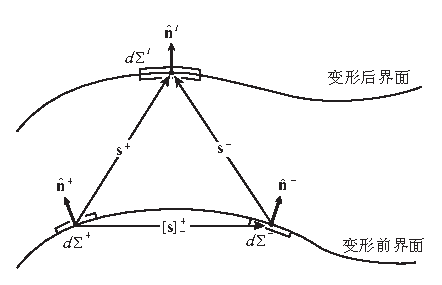
\includegraphics{../figures/chap03/fig03.eps}
\end{center}
\caption[slipbc]{\label{fig3.3}
%%%
一个滑动边界的局部示意图,包括形变之前(下图)和之后(上图)。初始面元$\hat{\bf n}^+d\/\Sigma^+$和$\hat{\bf n}^-d\/\Sigma^-$在$t$时刻合并成变形后的面元$\hat{\bf n}^td\/\Sigma^t$。确保这一点的一阶条件是${\bf r}={\bf x}^++{\bf s}^+={\bf x}^-+{\bf s}^-$。
%%%
}
\end{figure}
%%%
图~\ref{fig3.3}显示了一个滑动边界的局部;$\bnh^+d\/\Sigma^+$和$\bnh^-d\/\Sigma^-$分别为以变形前边界的正面和背面上的质点$\bx^+$和$\bx^-$为中心的两个初始面元。变形使两个质点$\bx^+$和$\bx^-$移动到同一点$\br$,两个面元$\bnh^+d\/\Sigma^+$和$\bnh^-d\/\Sigma^-$合并成变形后边界上相接的面元$\bnh^td\/\Sigma^t$。我们用上角标$\pm$表示在$\bx^{\pm}$处取值;例如,质点$\bx^{\pm}$的位移表示为$\bs^{\pm}$。一般的步骤是先将精确的关系式从$\br$转换到$\bx^{\pm}$,然后把在$\bx^+$与$\bx^-$两处的项用下式联系起来
%%%
\eq
\label{3.diffvec}
\bx^+-\bx^-=-[\bs]^+_-.
\en
%%%
由于仅精确到 $\|\bs\|$ 的一阶,因此究竟在变形前边界上何处计算~(\ref{3.diffvec})中的滑动$[\bs]^+_-$并不重要。
%%%

%%%
在移动后的点$\br$处精确的欧拉边界条件为
%%%
\eq
\label{3.stressbc}
[\bnh^td\/\Sigma^t\cdot\bT^{\rm E}]^+_-=\bzero,
\en
%%%
这里为方便起见,我们已将(连续的)微分面积$d\/\Sigma^t$代到公式~(\ref{2.stressbc})中。这一结果可以用第一类Piola-Kirchhoff应力的定义式~(\ref{2.TPKdef})写成变形前边界上的条件:
%%%
\eq
\label{3.exactbc}
\bnh^+d\/\Sigma^+\cdot(\bT^{0+}+\bT^{{\rm PK1}+})
=\bnh^-d\/\Sigma^-\cdot(\bT^{0-}+\bT^{{\rm PK1}-}).
\en
%%%
无穷小面积$d\/\Sigma^{\pm}$与$\bx^{\pm}$处单位法向$\bnh^{\pm}$之间的关系为
%%%
\eq
\label{3.dsigrel2}
d\/\Sigma^+-d\/\Sigma^-=-(\bdel^{\Sigma}\cdot[\bs]^+_-)_{\,}d\/\Sigma,
\en
\eq
\bnh^+-\bnh^-=(\bdel^{\Sigma}[\bs]^+_-)\cdot\bnh.
\en
%%%
此外,由于初始牵引力$\bnh\cdot\bT^0$是连续的,因此变化量$\bnh^+\cdot\bT^{0+}$和$\bnh^-\cdot\bT^{0-}$之间存在关系
%%%
\eq
\label{3.nT0cont}
\bnh^+\cdot\bT^{0+}-\bnh^-\cdot\bT^{0-}
=-[\bs]^+_-\cdot\bdel^{\Sigma}(\bnh\cdot\bT^0).
\en
%%%
同样地,由于精确到 $\|\bs\|$ 的一阶,究竟公式~(\ref{3.dsigrel2})--(\ref{3.nT0cont})右侧的$d\/\Sigma$是$d\/\Sigma^{\pm}$,或者$\bnh$是$\bnh^{\pm}$,或者$\bT^0$是$\bT^{0\pm}$,都是无关紧要的。利用~(\ref{3.dsigrel2})和~(\ref{3.nT0cont})对~(\ref{3.exactbc})进行简化,我们得到
%%%
\eq
\label{3.slipbc}
[\bnh\cdot\bT^{\rm PK1}-\bdel^{\Sigma}\cdot(\bs\,\bnh\cdot\bT^0)]^+_-
=\bzero.
\en
%%%
(\ref{3.slipbc})式是确保牵引力在任意滑动边界连续的线性化条件;在第5.3节中,我们将使用这个关系来得到理想化的地震断层的等效力表述。无滑动的密接边界可以被看作是滑动边界的特例;如果$\bs$是连续的,则~(\ref{3.slipbc})式必然退化为~(\ref{3.weldbc})。
%%%

\iffalse
On the fluid-solid boundaries $\Sigma_{\rm FS}$, the initial traction
is of the form
\fi
%%%
在固-液边界$\Sigma_{\rm FS}$上,初始牵引力的形式为
%%%
\eq
\label{3.nT0pi0}
\bnh\cdot\bT^0=-\varpi^0\bnh,
\en
%%%
其中$\varpi^0=-(\bnh\cdot\bT^0\cdot\bnh)$等于液态一侧的初始压强$p^0$。将~(\ref{3.nT0pi0})~代入~(\ref{3.slipbc})得到条件
%%%
\eq
\label{3.fsbc4}
[\bnh\cdot\bT^{\rm PK1}+\bdel^{\Sigma}\cdot(\varpi^0\bs\bnh)]^+_-=\bzero.
\en
%%%
经过一些整理之后,这一结果可以写成另一种形式
%%%
\eq
\label{3.fsbc3}
[\bnh\cdot\bT^{\rm PK1}+\bnh\,\bdel^{\Sigma}\cdot(\varpi^0\bs)
-\varpi^0(\bdel^{\Sigma}\bs)\cdot\bnh]^+_-=\bzero,
\en
%%%
这里我们使用了$\bnh\cdot\bs$和$\varpi^0$的连续性以及表面曲率张量的对称性:$(\bdel^{\Sigma}\bnh)^{\rm T}=\bdel^{\Sigma}\bnh$。(\ref{3.fsbc3})式是$\Sigma_{\rm FS}$上线性化动力学连续性条件的最有用的形式。
%%%

%%%
我们还需要条件~(\ref{2.stressfs})的线性化形式,即$\br$处的牵引力必须垂直于变形后的固-液边界:
%%%
\eq
\label{3.stressFS}
(\bnh^t\cdot\bT^{\rm E})\cdot(\bI-\bnh^t\bnh^t)=\bzero.
\en
%%%
(\ref{3.stressFS})式也可以改写为在变形前的边界 $\Sigma_{\rm FS}$ 上的公式
%%%
\eqa
\label{3.fsbc}
\lefteqn{
[-\varpi^{0\pm}\bnh^{\pm}+\bnh^{\pm}\cdot\bT^{{\rm PK1}\pm}]} \nonumber \\
& & \mbox{}\cdot\{\bI-[\bnh^{\pm}
-(\bdel^{\Sigma}\bs^{\pm})\cdot\bnh][\bnh^{\pm}-(\bdel^{\Sigma}
\bs^{\pm})\cdot\bnh]\}=\bzero.
\ena
%%%
精确到 $\|\bs\|$ 的一阶,这一条件等效于
%%%
\eq
\label{3.fsbc2}
[\bnh\cdot\bT^{\rm PK1}+\bnh\,\bdel^{\Sigma}\cdot(\varpi^0\bs)
-\varpi^0(\bdel^{\Sigma}\bs)\cdot\bnh]\cdot(\bI-\bnh\bnh)=\bzero,
\en
%%%
这里为方便起见,我们略去了已经无关紧要的上角标$\pm$,并增加了$\bnh\,\bdel^{\Sigma}\cdot(\varpi^0\bs)$一项。公式~(\ref{3.fsbc2})是确保固-液边界上没有切向牵引力的一阶关系式。比较~(\ref{3.fsbc3})~和~(\ref{3.fsbc2}),我们看到牵引力
%%%
\eq
\label{3.tPK1def}
\bt^{\rm PK1}=\bnh\cdot\bT^{\rm PK1}+\bnh\,\bdel^{\Sigma}\cdot(\varpi^0\bs)
-\varpi^0(\bdel^{\Sigma}\bs)\cdot\bnh
\en
%%%
是在$\Sigma_{\rm FS}$上连续的法向矢量:
%%%
\eq
\label{3.fsbc5}
[\bt^{\rm PK1}]^+_-=\bzero,
\en
\eq
\label{3.fsbc6}
\bt^{\rm PK1}=\bnh(\bnh\cdot\bt^{\rm PK1}).
\en
%%%
很容易验证公式~(\ref{3.fsbc5})在$\Sigma_{\rm SS}$上也是成立的;因此,法向条件~(\ref{3.fsbc6})是无摩擦的固-液边界与密接的固-固边界之间仅有的差别。
%%%

%%%
应用关系式~(\ref{3.TPK1TL1}),以上推导的所有条件都可以用拉格朗日柯西应力增量$\bT^{\rm L1}$ 来表示,而不是用$\bT^{\rm PK1}$;然而,我们并不需要这些结果。在第~\ref{3.sec.hydro}节中,我们将看到用$\bT^{\rm L1}$可以很方便地表示{\em 流体静力学\/}地球模型中的动力学边界条件。
%%%
\index{boundary conditions!dynamic|)}%

\subsection{引力边界条件}
\index{boundary conditions!gravitational|(}%

%%%
引力势函数和引力场微扰$\phi^{\rm E1}$和$\bg^{\rm E1}$的边界条件也是通过线性化变形后边界上精确的欧拉条件得到的。参照图~\ref{fig3.3},我们考虑边界上可能有切向滑动的普遍情况。
%%%

%%%
精确到 $\|\bs\|$ 的一阶,在变形后边界上具有位移的点$\br$处精确的连续性条件
%%%
\eq
[\phi^{\rm E}]^+_-=0,
\en
%%%
可以写为以下形式
%%%
\eq
\label{3.phiEbc1}
\phi^{0+}+\bs^+\cdot\bdel\phi^{0+}+\phi^{{\rm E1}+}=
\phi^{0-}+\bs^-\cdot\bdel\phi^{0-}+\phi^{{\rm E1}-},
\en
%%%
其中上角标$\pm$表示在$\bx^{\pm}$处取值。初始势函数$\phi^{0\pm}$由一阶展开式联系起来
%%%
\eq
\label{3.phiEbc2}
\phi^{0+}-\phi^{0-}=-[\bs]^+_-\cdot\bdel^{\Sigma}\phi^0.
\en
%%%
结合~(\ref{3.phiEbc1})~和~(\ref{3.phiEbc2}),我们得到简单的线性化条件
%%%
\eq
\label{3.phiEbc}
[\phi^{\rm E1}]^+_-=0.
\en
%%%
精确到 $\|\bs\|$ 的一阶,另一个精确的条件
%%%
\eq
[\bnh^t\cdot\bg^{\rm E}]^+_-=\bzero,
\en
%%%
可以写成
%%%
\eqa
\label{3.gEbc1}
\lefteqn{
[\bnh^+-(\bdel^{\Sigma}\bs^+)\cdot\bnh]\cdot[\bg^{0+}+\bs^+\cdot
\bdel\bg^{0+}+\bg^{{\rm E1}+}]} \nonumber \\
& & =[\bnh^--(\bdel^{\Sigma}\bs^-)\cdot\bnh]\cdot[\bg^{0-}+\bs^-\cdot
\bdel\bg^{0-}+\bg^{{\rm E1}-}].
\ena
%%%
$\bnh^{\pm}\cdot\bg^{0\pm}$也可以由类似于~(\ref{3.nT0cont})的展开式联系起来:
%%%
\eq
\label{3.ng0cont}
\bnh^+\cdot\bg^{0+}-\bnh^-\cdot\bg^{0-}
=-[\bs]^+_-\cdot\bdel^{\Sigma}(\bnh\cdot\bg^0).
\en
\iffalse
Upon combining~(\ref{3.gEbc1})~and~(\ref{3.ng0cont}) we obtain,
after some manipulation,
\fi
%%%
结合~(\ref{3.gEbc1})~和~(\ref{3.ng0cont}),经过一些推导,我们得到
%%%
\eq
\label{3.gEbc}
[\bnh\cdot\bdel\phi^{\rm E1}+4\pi G\rho^0\bnh\cdot\bs]^+_-=0.
\en
%%%
在推导~(\ref{3.gEbc})时,我们使用了泊松方程~(\ref{3.Poisson0})、$\phi^0$的连续性及其法向导数$\p_n\phi^0=\bnh\cdot\bdel\phi^0$, 以及拉普拉斯公式$\nabla^2=\bdel\cdot\bdel=\p_n^2+(\bdel\cdot\bnh)\p_n+
\bdel^{\Sigma}\cdot\bdel^{\Sigma}$。两个引力边界条件~(\ref{3.phiEbc})~和~(\ref{3.gEbc})在理想化的断层面及所有的$\Sigma=\p\earth\cup\Sigma_{\rm SS}\cup\Sigma_{\rm FS}$上都是成立的。
%%%

%%%
为方便起见,表~3.1完整地总结了$\Sigma$上的线性化边界条件。
%%%

%%%
\begin{table}[tb]
\label{table3.1}
\centering
\begin{tabular}{|l|l|} \hline
& \\
边界类型 & 线性化边界条件 \\
& \\ \hline
& \\
\index{boundary conditions!free surface}%
$\p\earth$: 自由表面 & $\bnh\cdot\bT^{\rm PK1}=\bzero$ \\
& \\
\index{boundary conditions!solid-solid}%
$\Sigma_{\rm SS}$: 固-固边界 & $[\bs]^+_-=\bzero$ \\
\vspace{-1.5 mm} & \vspace{-1.5 mm} \\
& $[\bnh\cdot\bT^{\rm PK1}]^+_-=\bzero$ \\
& \\
\index{boundary conditions!fluid-solid}%
$\Sigma_{\rm FS}$: 固-液边界 & $[\bnh\cdot\bs]^+_-=0$ \\
\vspace{-1.5 mm} & \vspace{-1.5 mm} \\
& $[\bt^{\rm PK1}]^+_-=\bnh[\bnh\cdot\bt^{\rm PK1}]^+_-=\bzero$ \\
& \\
$\Sigma$: 所有边界 & $[\phi^{\rm E1}]^+_-=0$ \\
\vspace{-1.5 mm} & \vspace{-1.5 mm} \\
& $[\bnh\cdot\bdel\phi^{\rm E1}+4\pi G\rho^0\,\bnh\cdot\bs]^+_-=0$ \\
& \\ \hline
\multicolumn{2}{|c|}{} \\
\multicolumn{2}{|c|}{$\bt^{\rm PK1}=\bnh\cdot\bT^{\rm PK1}
+\bnh\,\bdel^{\Sigma}\cdot(\varpi^0\bs)
-\varpi^0(\bdel^{\Sigma}\bs)\cdot\bnh$} \\
\multicolumn{2}{|c|}{} \\ \hline
\end{tabular}
\caption[bconds]{一般非流体静力学地球模型所满足的线性化的运动学、动力学和引力边界条件。}
\end{table}
%%%
\index{boundary conditions!gravitational|)}%

\renewcommand{\thesubsection}{$\!\!\!\raise1.3ex\hbox{$\star$}\!\!$
\arabic{chapter}.\arabic{section}.\arabic{subsection}}
\subsection{二阶切向滑动条件}
\index{boundary conditions!second-order|(}%
\label{3.sec.slipbc}
\renewcommand{\thesubsection}{\arabic{chapter}.\arabic{section}.\arabic{subsection}}

%%%
在第~3.9.4节中,我们需要一个{\em 二阶\/}切向滑动条件来计算具有固-液边界的地球模型,在变形后该模型所储存的弹性能。这一条件的获得可以通过对精确的欧拉连续性条件
%%%
\eq
\label{3.ndotuEbc}
[\bnh^t\cdot\bu^{\rm E}]^+_-=0
\en
%%%
做展开,然后保留到二阶项 $\|\bs\|^2$。精确到 $\|\bs\|$ 的二阶, 我们可以将~(\ref{3.ndotuEbc})式用相应的位于 $\bx^{\pm}$ 的拉格朗日速度$\p_t\bs^{\pm}$ 写成
%%%
\eq
\label{3.slipsq}
[\bnh^+-(\bdel^{\Sigma}\bs^+)\cdot\bnh]\cdot\p_t\bs^+
=[\bnh^--(\bdel^{\Sigma}\bs^-)\cdot\bnh]\cdot\p_t\bs^-,
\en
%%%
\bnh^{\pm}\cdot\p_t\bs^{\pm}$由类似于~(\ref{3.nT0cont})的表达式联系起来:
%%%
\eq
\label{3.slipsq4}
\bnh^+\cdot\p_t\bs^+-\bnh^-\cdot\p_t\bs^-=
[\bnh\cdot\p_t\bs-\bs\cdot\bdel^{\Sigma}(\bnh\cdot\p_t\bs)]^+_-,
\en
%%%
其中我们保留了一阶项 $[\bnh\cdot\p_t\bs]^+_-$。结合(\ref{3.slipsq})和(\ref{3.slipsq4})式,我们看到
%%%
\eqa
\label{3.slipsq2}
\lefteqn{[\bnh\cdot\p_t\bs-\p_t\bs\cdot\bdel^{\Sigma}
(\bnh\cdot\bs)-\bs\cdot\bdel^{\Sigma}(\bnh\cdot\p_t\bs)
+\p_t\bs\cdot(\bdel^{\Sigma}\bnh)\cdot\bs]^+_-} \nonumber \\
& & =\p_t[\bnh\cdot\bs-\bs\cdot\bdel^{\Sigma}(\bnh\cdot\bs)
+\half\bs\cdot(\bdel^{\Sigma}\bnh)\cdot\bs]^+_-=0,
\ena
%%%
这里我们使用了对称性$(\bdel^{\Sigma}\bnh)^{\rm T}=\bdel^{\Sigma}\bnh$来得到第二个等式。对~(\ref{3.slipsq2})积分,并使用初始条件$\bs(\bx,0)=\bzero$来消去未定常数,我们得到最终结果:
%%%
\eq
\label{3.slipsq3}
[\bnh\cdot\bs-\bs\cdot\bdel^{\Sigma}(\bnh\cdot\bs)
+\half\bs\cdot(\bdel^{\Sigma}\bnh)\cdot\bs]^+_-=0.
\en
%%%
(\ref{3.slipsq3})式是确保边界两侧物质没有分离或互相穿透的二阶条件;它既适用于固-固断层面,也适用于固-液边界$\Sigma_{\rm FS}$。
%%%
\index{boundary conditions!second-order|)}%
\index{boundary conditions!linearized|)}%

\section{线性化的势理论}
\index{gravitational potential theory|(}%

\label{3.sec.grav}

%%%
有两种方法可以建立引力微扰$\phi^{\rm E1}$、$\bg^{\rm E1}$、$\phi^{\rm L1}$和$\bg^{\rm L1}$与位移$\bs$之间的关系。我们在这里对两种方法都加以考虑,并证明它们是等价的。
%%%
\index{gravitational perturbation}%
\index{perturbation!gravitational}%

\subsection{线性化的泊松方程}
\index{Poisson's equation|(}%

%%%
欧拉势函数微扰$\phi^{\rm E1}$是线性化的泊松方程
%%%
\eq
\label{3.Poisson}
\nabla^2\phi^{\rm E1}=4\pi G\rho^{\rm E1},
\en
%%%
满足前面推导出的边界条件
%%%
\eq
\label{3.surfmass}
[\phi^{\rm E1}]^+_-=0,\qquad
[\bnh\cdot\bdel\phi^{\rm E1}]^+_-=-4\pi G[\rho^0]^+_-(\bnh\cdot\bs).
\en
%%%
的解。微扰方程~(\ref{3.Poisson})可以直接在~(\ref{2.poisson})中消去初始方程~(\ref{3.Poisson0}) 而得到。在地球以外$\rho^{\rm E1}=0$,故势函数微扰是调和的:$\nabla^2\phi^{\rm E1}=0$。线性化边界值问题~(\ref{3.Poisson})--(\ref{3.surfmass})中所有的量都有简单的物理解释;特别是$-[\rho^0]^+_-(\bnh\cdot\bs)$,它是因边界$\Sigma$的法向位移而产生的{\em 质量的表观表面密度\/}。(\ref{3.Poisson})的解$\phi^{\rm E1}$显然是
%%%
\eq
\label{3.phiE1int}
\phi^{\rm E1}=-G\int_{\subearth}\frac{\rho^{{\rm E1}\prime}}
{\|\bx-\bx'\|}\,dV'
+G\int_{\Sigma}\frac{[\rho^{0\prime}]^+_-
(\bnh^{\prime}\cdot\bs')}{\|\bx-\bx'\|}\,d\/\Sigma',
\en
%%%
其中第一项来自$\earth$中的体积密度微扰$\rho^{\rm E1}$,第二项则来自表观表面质量微扰。将$\rho^{{\rm E1}\prime}=-\bdel^{\prime}
\cdot(\rho^{0\prime}\bs')$代入公式~(\ref{3.phiE1int}),并应用高斯定理,我们发现面积分相消,而仅剩下
%%%
\eq
\label{3.phiE1int2}
\phi^{\rm E1}=
-G\int_{\subearth}\frac{\rho^{0\prime}\bs'\cdot
(\bx-\bx')}{\|\bx-\bx'\|^3}\,dV'.
\en
%%%
由于被积函数中的密度$\rho^0$在$\Sigma$上可能是不连续的,因此有必要将高斯定理分别应用于$\earth$中每个部分的体积,并将其结果相加。(\ref{3.phiE1int2})式是欧拉势函数微扰$\phi^{\rm E1}$作为质点位移$\bs$的线性泛函的最简便的解析表达式。其相应的欧拉引力增量$\bg^{\rm E1}=-\bdel\phi^{\rm E1}$可以写为
%%%
\eq
\label{3.gE1int}
\bg^{\rm E1}=G\int_{\subearth}
\rho^{0\prime}(\bs'\cdot\bPi)\,dV',
\en
\index{gravitational potential!Eulerian}%
%%%
其中
%%%
\eq
\label{3.bPidef}
\bPi=\frac{\bI}{\|\bx-\bx'\|^3}
-\frac{3(\bx-\bx')(\bx-\bx')}{\|\bx-\bx'\|^5}.
\en
%%%
借助~(\ref{3.phiEL1}),可以建立拉格朗日微扰$\phi^{\rm L1}$和$\bg^{\rm L1}$与$\phi^{\rm E1}$和$\bg^{\rm E1}$之间的关系。
%%%
\index{Poisson's equation|)}%

\subsection{线性化的积分关系}

%%%
我们也可以用另外一种方式,将精确的积分关系~(\ref{2.phiEint})--(\ref{2.gLint})线性化来得到$\phi^{\rm E1}$、$\bg^{\rm E1}$、$\phi^{\rm L1}$和$\bg^{\rm L1}$。以~(\ref{2.phiLint})为例,我们将其改写为
%%%
\eq
\phi^0+\phi^{\rm L1}=-G\int_{\subearth}\frac{\rho^{0\prime}}
{\|\bx+\bs-\bx'-\bs'\|}\,dV',
\en
%%%
并将其右边以$\bs$和$\bs'$的幂级数展开,可得到零阶项就是$\phi^0$,而一阶项则为
%%%
\eq
\label{3.phiLint}
\phi^{\rm L1}=
-G\int_{\subearth}\frac{\rho^{0\prime}(\bs'-\bs)\cdot
(\bx-\bx')}{\|\bx-\bx'\|^3}\,dV'.
\en
%%%
可以看到,该式正好就是$\phi^{\rm L1}=\phi^{\rm E1}+\bs\cdot\bdel\phi^0$,其中$\phi^{\rm E1}$由~(\ref{3.phiE1int2})给定。将下式展开
%%%
\eq
\bg^0+\bg^{\rm L1}
=-G\int_{\subearth}\frac{\rho^{0\prime}
(\bx+\bs-\bx'-\bs')}
{\|\bx+\bs-\bx'-\bs'\|^3}\,dV'
\en
%%%
同样会导致
%%%
\eq
\bg^{\rm L1}=G\int_{\subearth}
\rho^{0\prime}[(\bs'-\bs)\cdot\bPi]\,dV',
\en
\index{gravitational potential!Lagrangian}%
%%%
上式与$\bg^{\rm L1}=\bg^{\rm E1}+\bs\cdot\bdel\bg^0=-\bdel\phi^{\rm E1}-\bs\cdot\bdel
\bdel\phi^0$完全相同。
%%%
 
\renewcommand{\thesubsection}{$\!\!\!\raise1.3ex\hbox{$\star$}\!\!$
\arabic{chapter}.\arabic{section}.\arabic{subsection}}
\subsection{引力应力张量增量}
\index{tensor!gravitational stress|(}%
\index{gravitational stress tensor|(}%
\index{stress!gravitational|(}%
\index{stress!incremental|(}%
\renewcommand{\thesubsection}{\arabic{chapter}.\arabic{section}.\arabic{subsection}}

%%%
在第~2.8.3节中定义的引力应力张量可以分解为初始应力和一阶微扰:
%%%
\eq \label{3.gstress1}
\bN^{\rm E}=\bN^0+\bN^{\rm E1},\qquad
\bN^{\rm PK}=\bN^0+\bN^{\rm PK1},
\en
%%%
其中
%%%
\eq \label{3.gstress2}
\bN^0=(8\pi G)^{-1}[(\bg^0\cdot\bg^0)\bI
-2\bg^0\bg^0].
\en
%%%
欧拉应力增量显然是
%%%
\eq \label{3.gstress3}
\bN^{\rm E1}=(4\pi G)^{-1}[(\bg^0\cdot\bg^{\rm E1})\bI
-\bg^0\bg^{\rm E1}-\bg^{\rm E1}\bg^0],
\en
%%%
通过与~(\ref{3.TL1TE1rel})和~(\ref{3.TPK1TL1})类比,第一类Piola-Kirchhoff应力增量则是
%%%
\index{stress!first Piola-Kirchhoff}%
\index{Piola-Kirchhoff stress!first}%
\eq
\bN^{\rm PK1}=\bN^{\rm E1}+\bs\cdot\bdel\bN^0+\bN^0(\bdel\cdot\bs)-
(\bdel\bs)^{\rm T}\cdot\bN^0,
\en
%%%
很容易验证如下结果
%%%
\eq
\bdel\cdot\bN^{\rm E1}=
\rho^0\bg^{\rm E1}+\rho^{\rm E1}\bg^0,\qquad
\bdel\cdot\bN^{\rm PK1}=\rho^0\bg^{\rm L1}.
\en
%%%
因此,线性化动量方程~(\ref{3.momeqn})或~(\ref{3.lagmomeqn})可以用下面两种形式中的任何一种来表示
%%%
\eqa \label{3.gstress4} \lefteqn{
\rho^0[\p_t^2\bs+2\bOmega\times\p_t\bs+\bOmega\times(\bOmega\times\bs)]
=\bdel\cdot(\bT^{\rm E1}+\bN^{\rm E1})} \nonumber \\
&&\mbox{}\hspace{44.8 mm}=\bdel\cdot(\bT^{\rm PK1}+\bN^{\rm PK1}).
\ena
%%%
变形后边界上的引力牵引力所满足的的精确的欧拉连续性条件$[\bnh^t d\/\Sigma^t\cdot\bN^{\rm E}]^+_-=\bzero$可遵循第~3.4.2节中的步骤线来进行性化;类似于~(\ref{3.slipbc})式,这样得到的变形前边界上的一阶关系为
%%%
\eq \label{3.gstress6}
[\bnh\cdot\bN^{\rm PK1}-\bdel^{\Sigma}\cdot(\bs\,\bnh\cdot\bN^0)]^+_-
=\bzero.
\en
%%%
(\ref{3.gstress6})在密接和滑动边界上的任何一点都必须成立,该式也可以直接从势函数和引力边界条件~(\ref{3.phiEbc})和~(\ref{3.gEbc})得到。
%%%
\index{tensor!gravitational stress|)}%
\index{gravitational stress tensor|)}%
\index{stress!gravitational|)}%
\index{gravitational potential theory|)}%
\index{stress!incremental|)}%

\section{线性化的弹性本构关系}
\index{constitutive relation!elastic|(}%
\index{elastic constitutive relation|(}%
\index{stress-strain relation|(}%
\index{stress!incremental|(}%
\label{3.sec.constrel}

%%%
到目前为止,我们在本章中得到的所有结果都可以视为是线性化的几何或物理定律。要使这些公式完备化还必须要有应力增量$\bT^{\rm L1}$、$\bT^{\rm PK1}$和$\bT^{\rm SK1}$与位移梯度$\bdel\bs$之间的线性化的本构关系。如第~2.10节所述,我们目前暂且假设组成地球的物质是绝热且完全弹性的。我们在第六章会将这里的结果推广到线性非弹性地球模型的情形。
%%%

\subsection{弹性应变能密度}
\index{energy!strain|(}%
\index{strain energy|(}%

%%%
根据定义,绝热、完全弹性物质的拉格朗日内能体积密度$\rho^0U^{\rm L}$仅依赖于局地拉格朗日应变张量$\bE^{\rm L}$。在自洽的线性理论中,能量的计算必须精确到$\|\bs\|$的二阶;这就使得在能量分析中不可能使用线性化的近似$\bE^{\rm L}=\beps$。在给定$\rho^0U^{\rm L}$时,我们必须使用$\bE^{\rm L}$和$\bdel\bs$之间的精确关系:
%%%
\eq
\label{3.ELexact}
\bE^{\rm L}=\half[\bdel\bs+(\bdel\bs)^{\rm T}]
+\half(\bdel\bs)\cdot(\bdel\bs)^{\rm T}.
\en
%%%
在下面的大部分讨论中,使用坐标不变量的符号会使公式变得十分繁琐,因此我们会经常采用角标符号;用笛卡尔坐标系$\bxh_1$,$\bxh_2$,$\bxh_3$ 中的分量形式表示的(\ref{3.ELexact})式为
%%%
\eq
E^{\rm L}_{ij}=\half(\p_is_j+\p_js_i)+\half\p_is_{k\,}\p_js_k.
\en
%%%
将弹性能密度对应变$\bE^{\rm L}$的依赖关系展开到$\|\bs\|$的二阶,我们将$\rho^0U^{\rm L}$写为
%%%
\eqa
\label{3.elen}
\lefteqn{\rho^0U^{\rm L}=\rho^0U^0+\bT^0\!:\!\bE^{\rm L}
+\half\bE^{\rm L}\!:\!\bXi\!:\!\bE^{\rm L}} \nonumber \\
&&\mbox{}\hspace{0.9 mm}=\rho^0U^0+T^{\,0}_{ij\,}E^{\rm L}_{ij}+\half
E^{\rm L}_{ij\,}\Xi_{\,ijkl\,}E^{\rm L}_{kl},
\ena
%%%
其中$\bXi$是一个四阶张量。零阶项$\rho^0U^0$是变形前参考构形中的内能密度;接着的两项分别来自$\rho^0U^{\rm L}$对应变的一阶和二阶依赖关系。式~(\ref{3.elen})中一阶展开系数的选择必须满足确保在精确到 $\|\bs\|$ 的零阶时,所有三个应力$\bT^{\rm L}$、$\bT^{\rm PK}$和$\bT^{\rm SK}$都退化为初始应力$\bT^0$。不失一般性,可以假定四阶张量$\bXi$的分量$\Xi_{\,ijkl}$满足对称关系
%%%
\eq
\label{3.Xisym}
\Xi_{\,ijkl}=\Xi_{\,jikl}=\Xi_{\,ijlk}=\Xi_{\,klij}.
\en

%%%
第二类Piola-Kirchhoff应力$\bT^{\rm SK}$可以由公式~(\ref{2.TSKofE})用能量密度$\rho^0U^{\rm L}$定义为:
%%%
\index{stress!second Piola-Kirchhoff}%
\index{Piola-Kirchhoff stress!second}%
\eq
\label{3.TSKstrain}
\bT^{\rm SK}=\bT^0+\bT^{\rm SK1}=\rho^0\!\left(\frac{\p U^{\rm L}}
{\p\bE^{\rm L}}\right)
=\bT^0+\bXi\!:\!\bE^{\rm L}.
\en
%%%
将展开式~(\ref{3.elen})对$\bE^{\rm L}$做两次微分,我们得到张量$\bXi$的分量的显式公式:
%%%
\eq
\Xi_{\,ijkl}=\rho^0\!\left(\frac{\p^2 U^{\rm L}}
{\p_{\!}E^{\rm L}_{ij} \,\p_{\!}E^{\rm L}_{kl}}\right).
\en
%%%
等式$\Xi_{\,ijkl}=\Xi_{\,klij}$可以被看作是$\rho^0U^{\rm L}$的混合偏导数相等的结果。这些在热力学中普遍存在的关系被称为{\em 麦克斯韦关系}。
\index{Maxwell relation}%
一旦有了线性关系~(\ref{3.TSKstrain}),就可以将$\bE^{\rm L}$用无穷小应变张量$\beps$来替换,并且在 $\|\bs\|$ 的一阶精度下将第二类Piola-Kirchhoff应力增量$\bT^{\rm SK1}$的本构关系写为
%%%
\eq
\label{3.TSK1strain}
\bT^{\rm SK1}=\bXi\!:\!\beps,
\en
%%%
或者等价为$T^{\rm SK1}_{ij}=\Xi_{\,ijkl\,}\varepsilon_{kl}$。
\vspace{-0.8 mm} 
但是,我们不能在弹性应变能密度~(\ref{3.elen})中将$\bE^{\rm L}$用$\beps$做类似的替换,因为在$\|\bs\|$的二阶精度下$\bT^0\!:\!\bE^{\rm L}$不等于$\bT^0\!:\!\beps$。
%%%

%%%
利用关系式~(\ref{3.TPK1TL1})--(\ref{3.TPK1TSK1}),可借由~(\ref{3.TSK1strain})得到第一类Piola-Kirchhoff应力增量$\bT^{\rm PK1}$
\index{stress!first Piola-Kirchhoff}%
\index{Piola-Kirchhoff stress!first}%
和拉格朗日柯西应力增量$\bT^{\rm L1}$的线性化本构关系。
\index{stress!Cauchy}%
\index{Cauchy stress}%
结果的最简便的表达式是用两个新的四阶张量$\bLambda$和$\bUpsilon$:
%%%
\eq
\label{3.TPK1grads}
\bT^{\rm PK1}=\bLambda\!:\!\bdel\bs,
\en
\eq
\label{3.TL1grads}
\bT^{\rm L1}=\bUpsilon\!:\!\bdel\bs,
\en
%%%
或者等价于$T^{\rm PK1}_{ij}=\Lambda_{ijkl\,}\p_ks_l$,$T^{\rm L1}_{ij}=\Upsilon_{ijkl\,}\p_ks_l$。$\bLambda$和$\bUpsilon$的分量可以用$\bXi$的分量定义
%%%
\eq
\label{3.LamXi}
\Lambda_{\,ijkl}=\Xi_{\,ijkl}+T^{\,0}_{ik\,}\delta_{jl},
\en
\eqa
\label{3.GamXi}
\lefteqn{
\Upsilon_{ijkl}=\Lambda_{ijkl}+T^{\,0}_{jk\,}\delta_{il}
-T^{\,0}_{ij\,}\delta_{kl}
} \nonumber \\
& & \;\,=\Xi_{\,ijkl}+T^{\,0}_{ik\,}\delta_{jl}
+T^{\,0}_{jk\,}\delta_{il}-T^{\,0}_{ij\,}\delta_{kl},
\ena
%%%
其中$\delta_{ij}$是克罗内克符号。从~(\ref{3.Xisym}) 和~(\ref{3.LamXi})--(\ref{3.GamXi})可以看到,$\Lambda_{ijkl}$和$\Upsilon_{ijkl}$的分量满足对称关系
%%%
\eq
\label{3.Lamsym}
\Lambda_{ijkl}=\Lambda_{klij},
\en
\eq
\label{3.Gamsym}
\Upsilon_{ijkl}=\Upsilon_{jikl}.
\en

%%%
将~(\ref{3.ELexact})式~代入~(\ref{3.elen}),并使用~(\ref{3.LamXi}),我们发现在$\|\bs\|$的二阶精度下弹性能密度$\rho^0U^{\rm L}$可以改写为
%%%
\eqa
\label{3.elen3}
\lefteqn{\rho^0U^{\rm L}=\rho^0U^0+\bT^0\!:\!\beps+
\half\bdel\bs\!:\!\bLambda\!:\!\bdel\bs} \nonumber \\
&&\mbox{}\,\,=\rho^0U^0+T^{\,0}_{ij\,}\varepsilon_{ij}
+\half\p_is_{j\,}\Lambda_{ijkl\,}\p_ks_l.
\ena
%%%
将~(\ref{3.TPK1grads})~和~(\ref{3.elen3})做比较,我们可以用类似于~(\ref{3.TSKstrain})的方式将第一类Piola-Kirchhoff应力$\bT^{\rm PK}$ 写为:
%%%
\index{stress!first Piola-Kirchhoff}%
\index{Piola-Kirchhoff stress!first}%
\eq
\label{3.TPKderiv}
\bT^{\rm PK}=\bT^0+\bT^{\rm PK1}=\rho^0\!\left[\frac{\p U^{\rm L}}
{\p(\bdel\bs)}\right].
\en
%%%
(\ref{3.TPKderiv})是普遍关系~(\ref{2.TPKofF})的线性化形式。利用之前得到的$\bF^{\rm T}=\bI+\bdel\bs$和链式法则,我们可以确认$\p U^{\rm L}\hspace{-0.4 mm}/\p\bF^{\rm T}
=\p U^{\rm L}\hspace{-0.4 mm}/\p(\bdel\bs)$。将(\ref{3.elen3})对位移梯度$\bdel\bs$微分两次,我们看到张量$\bLambda$的分量可以写为
%%%
\eq
\Lambda_{ijkl}=\rho^0\!\left[\frac{\p^2 U^{\rm L}}
{\p(\p_is_j)_{\,}\p(\p_ks_l)}\right].
\en
%%%
$\Lambda_{ijkl}=\Lambda_{klij}$这一重要的对称关系是弹性麦克斯韦关系的又一个实例。
%%%
\index{Maxwell relation}%

%%%
如果在一开始将$\rho^0U^{\rm L}$写成~(\ref{3.elen3})而不是~(\ref{3.elen})的形式,我们本可以避免引入第二类Piola-Kirchhoff应力张量$\bT^{\rm SK}$。(\ref{3.elen})的优点在于它明确地符合物质参照系无关原理。
\index{frame indifference}%
\index{material frame indifference}%
为确保~(\ref{3.elen})的表述不依赖于转动张量$\bQ$,我们必须要求它满足~(\ref{2.UofFconstr})的约束。在 $\|\bs\|$ 的一阶精度下,这会导致如下两个条件
%%%
\eq
\Lambda_{jikl}-\Lambda_{ijkl}=T^{\,0}_{jk\,}\delta_{il}
-T^{\,0}_{ik\,}\delta_{jl},
\en
\eq
\Lambda_{ijlk}-\Lambda_{ijkl}=T^{\,0}_{il\,}\delta_{jk}
-T^{\,0}_{ik\,}\delta_{jl}.
\en
%%%
在目前的推导中,上述条件连同下面$\bUpsilon$的相应结果,
%%%
\eq
\Upsilon_{ijlk}-\Upsilon_{ijkl}=T^{\,0}_{il\,}\delta_{jk}
-T^{\,0}_{ik\,}\delta_{jl}+T^{\,0}_{jl\,}\delta_{ik}
-T^{\,0}_{jk\,}\delta_{il},
\en
\eq
\Upsilon_{klij}-\Upsilon_{ijkl}=T^{\,0}_{il\,}\delta_{jk}
-T^{\,0}_{jk\,}\delta_{il}+T^{\,0}_{ij\,}\delta_{kl}
-T^{\,0}_{kl\,}\delta_{ij},
\en
%%%
是关系式~(\ref{3.LamXi})--(\ref{3.GamXi})和张量$\bXi$的对称性~(\ref{3.Xisym})的直接结果。
%%%
\index{energy!strain|)}%
\index{strain energy|)}%

\subsection{弹性张量}
\index{tensor!elastic|(}%
\index{elastic tensor|(}%

%%%
在没有任何初始应力$\bT^0$的情况下,经典线性弹性应力应变关系为
%%%
\eq
\label{3.classHooke}
\bT=\bGamma\!:\!\beps,
\en
%%%
其中$\bT$可以解释为$\bT^{\rm L}$或$\bT^{\rm E}$,且$\bGamma$满足
%%%
\eq
\label{3.Csym}
\Gamma_{ijkl}=\Gamma_{jikl}=\Gamma_{ijlk}=\Gamma_{klij}.
\en
%%%
公式~(\ref{3.classHooke})通常被称为{\em 胡克定律\/};
\index{Hooke's law}%
(\ref{3.Csym})是具有21个独立系数的四阶{\em 弹性张量}的经典对称关系。
\index{elastic tensor}%
而对于有应力增量叠加在零阶初始应力$\bT^0$上这一更普遍的情形,我们会发现将$\bXi$, $\bLambda$ 和 $\bUpsilon$用$\bT^0$和具有弹性对称关系~(\ref{3.Csym})的张量$\bGamma$来表示是有益的。根据~(\ref{3.Xisym}),张量$\bXi$已经满足这些对称关系,因此~(\ref{3.LamXi})和~(\ref{3.GamXi})这些关系是所期望的类型;然而,$\bXi$却不是最能满足我们目的的弹性张量。
%%%

%%%
事实上,我们在弹性张量的选择上有相当大的自由度;唯一的要求是满足~(\ref{3.Xisym})和~(\ref{3.Lamsym})--(\ref{3.Gamsym})这三组对称关系以及相互之间的关系~(\ref{3.LamXi})--(\ref{3.GamXi})。很容易验证具有以下形式的张量$\bXi$,$\bLambda$和$\bUpsilon$满足所有上述条件
%%%
\eqa
\label{3.XiT}
\lefteqn{
\Xi_{\,ijkl}=\Gamma_{ijkl}+a(T^{\,0}_{ij\,}\delta_{kl}
+T^{\,0}_{kl\,}\delta_{ij})} \\
& & \mbox{}\qquad\qquad\!\!+b(T^{\,0}_{ik\,}\delta_{jl}+T^{\,0}_{jk\,}
\delta_{il}+T^{\,0}_{il\,}\delta_{jk}+T^{\,0}_{jl\,}\delta_{ik}), \nonumber 
\ena
\eqa
\label{3.LamT}
\lefteqn{
\Lambda_{\,ijkl}=\Gamma_{ijkl}+a(T^{\,0}_{ij\,}
\delta_{kl}+T^{\,0}_{kl\,}\delta_{ij})} \\
& & \mbox{}\qquad\qquad\!\!+(1+b)T^{\,0}_{ik\,}\delta_{jl}+b
(T^{\,0}_{jk\,}\delta_{il}
+T^{\,0}_{il\,}\delta_{jk}+T^{\,0}_{jl\,}\delta_{ik}), \nonumber 
\ena
\eqa
\label{3.GamT}
\lefteqn{
\Upsilon_{ijkl}=\Gamma_{ijkl}+(a-1)T^{\,0}_{ij\,}\delta_{kl}
+aT^{\,0}_{kl\,}\delta_{ij}} \\
& & \mbox{}\qquad\qquad\!\!+(1+b)
(T^{\,0}_{ik\,}\delta_{jl}+T^{\,0}_{jk\,}\delta_{il})
+b(T^{\,0}_{il\,}\delta_{jk}+T^{\,0}_{jl\,}\delta_{ik}), \nonumber 
\ena
%%%
其中$\Gamma_{ijkl}=\Gamma_{jikl}=\Gamma_{ijlk}=\Gamma_{klij}$,$a$和$b$为任意标量。(\ref{3.XiT})中括号内与$a$和$b$相乘的两个表达式是两个仅有的能满足弹性对称关系的$\bT^0\bI$排列的线性组合。每一组标量$a$和$b$的选择都定义了一个可能的弹性张量$\bGamma$。其中最方便的选择是\textcite{dahlen72}所采用的:
%%%
\eq
a=-b=\half.
\en
%%%
该选择所得到的张量$\bXi$,$\bLambda$和$\bUpsilon$为
%%%
\eqa
\label{3.XiT2}
\lefteqn{
\Xi_{\,ijkl}=\Gamma_{ijkl}+\half(T^{\,0}_{ij\,}
\delta_{kl}+T^{\,0}_{kl\,}
\delta_{ij}} \nonumber  \\
& & \mbox{}\qquad\qquad\qquad-T^{\,0}_{ik\,}\delta_{jl}-T^{\,0}_{jk\,}\delta_{il}
-T^{\,0}_{il\,}\delta_{jk}-T^{\,0}_{jl\,}\delta_{ik}),
\ena
\eqa
\lefteqn{
\label{3.LamT2}
\Lambda_{\,ijkl}=\Gamma_{ijkl}+\half(T^{\,0}_{ij\,}\delta_{kl}
+T^{\,0}_{kl\,}\delta_{ij}} \nonumber  \\
& & \mbox{}\qquad\qquad\qquad+T^{\,0}_{ik\,}\delta_{jl}-T^{\,0}_{jk\,}\delta_{il}
-T^{\,0}_{il\,}\delta_{jk}-T^{\,0}_{jl\,}\delta_{ik}),
\ena
\eqa
\label{3.GamT2}
\lefteqn{
\Upsilon_{ijkl}=\Gamma_{ijkl}+\half(-T^{\,0}_{ij\,}\delta_{kl}
+T^{\,0}_{kl\,}
\delta_{ij}} \nonumber  \\
& & \mbox{}\qquad\qquad\qquad+T^{\,0}_{ik\,}\delta_{jl}+T^{\,0}_{jk\,}\delta_{il}
-T^{\,0}_{il\,}\delta_{jk}-T^{\,0}_{jl\,}\delta_{ik}).
\ena

%%%
将公式~(\ref{3.XiT2})--(\ref{3.GamT2})及分解式$\bT^0=-p^0\bI+\btau^0$和$(\bdel\bs)^{\rm T}=\beps+\bomega$代入表达式~(\ref{3.TSK1strain})--(\ref{3.TL1grads}),我们可以将应力增量$\bT^{\rm SK1}$、$\bT^{\rm PK1}$和$\bT^{\rm L1}$写为
%%%
\eqa
\label{3.TSK1all}
\lefteqn{
T^{\rm SK1}_{ij}=\Gamma_{ijkl\,}\ep_{kl}+p^0(2\ep_{ij}
-\ep_{kk\,}\delta_{ij})} \nonumber \\
& & \mbox{}\qquad\qquad\;\;\;\,+\half(\tau^0_{ij\,}\ep_{kk}
+\tau^0_{kl\,}\ep_{kl\,}\delta_{ij})
-\ep_{ik\,}\tau^0_{kj}-\tau^0_{ik\,}\ep_{kj},
\ena
\eqa
\label{3.TPK1all}
\lefteqn{
T^{\rm PK1}_{ij}=\Gamma_{ijkl\,}\ep_{kl}+p^0(\ep_{ij}+\omega_{ij}
-\ep_{kk\,}\delta_{ij})} \nonumber  \\
& & \mbox{}\qquad\qquad\;\;\;_{\,}
+\half(\tau^0_{ij\,}\ep_{kk}+\tau^0_{kl\,}\ep_{kl\,}\delta_{ij})
-\ep_{ik\,}\tau^0_{kj}-\tau^0_{ik\,}\omega_{kj},
\ena
\eq
\label{3.TL1all}
T^{\rm L1}_{ij}=\Gamma_{ijkl\,}\ep_{kl}
+\half(-\tau^0_{ij\,}\ep_{kk}+\tau^0_{kl\,}\ep_{kl\,}\delta_{ij})
+\omega_{ik\,}
\tau^0_{kj}-\tau^0_{ik\,}\omega_{kj}.
\en
%%%
(\ref{3.TSK1all})、~(\ref{3.TPK1all})~和~(\ref{3.TL1all})分别是普遍结果~(\ref{2.TSKofR})、~(\ref{2.TPKofR})--(\ref{2.TPKofR2})和(\ref{2.TLofR})--(\ref{2.TLofR2})的线性化形式。这些关系一并构成了胡克定律在具有预应力弹性介质中的推广;$\bT^{\rm SK1}$、$\bT^{\rm PK1}$和$\bT^{\rm L1}$对初始压强$p^0$和偏应力$\btau^0$以及对应变和转动张量$\beps$和$\bomega$的依赖性是明显的。值得注意的是,拉格朗日柯西应力增量$\bT^{\rm L1}$并不显性地依赖于初始压强$p^0$,而仅依赖于弹性张量$\bGamma$和初始偏应力$\btau^0$。事实上,这也是促使我们在~(\ref{3.XiT})--(\ref{3.GamT})中取$a=-b=1/2$的原因;因为只有这一选择完全消除了$\bT^{\rm L1}$对$p^0$的显性依赖。完整的拉格朗日柯西应力$\bT^{\rm L}=\bT^0+\bT^{\rm L1}$可以用坐标不变量符号写为
%%%
\index{stress!Cauchy}%
\index{Cauchy stress}%
\eqa
\label{3.TLinterpr}
\lefteqn{
\bT^{\rm L}=\overbrace{-p^0\bI+\btau^0+\bomega
\cdot\btau^0-\btau^0\cdot\bomega}^{\mbox{\scriptsize 转动后的初始应力}}}
\nonumber \\
& & \mbox{}\qquad\qquad
+\underbrace{\bGamma\!:\!\beps-\half\btau^0({\rm tr}\,\beps)
+\half(\btau^0\!:\!\beps)\bI}_{\mbox{\scriptsize 依赖于应变的应力}}.
\ena
%%%
(\ref{3.TLinterpr})中的前四项可以被看出是{\em 转动后的初始应力}$\bQ^{\rm T}\cdot\bT^0\cdot\bQ$,其余几项表示应变$\beps$引起的应力微扰。
%%%

%%%
根据定义,各向同性固体的弹性张量为
%%%
\eq
\label{3.isoGamdef}
\Gamma_{ijkl}=(\kappa-\twothirds\mu)\delta_{ij\,}\delta_{kl}+
\mu(\delta_{ik\,}\delta_{jl}+\delta_{il\,}\delta_{jk}),
\en
%%%
其中$\kappa$是等熵{\em 不可压缩性\/}或体变模量,$\mu$是{\em 刚度\/}或切变模量。近似式~(\ref{3.isoGamdef})最常用于$\btau^0=\bzero$的{\em 流体静力学\/}地球模型。在各向同性流体静力学模型中,拉格朗日柯西应力增量可以表示为$\bT^{\rm L1}=-p^{\rm L1}\bI+\btau^{\rm L1}$,其中$p^{\rm L1}=-\kappa(\bdel\cdot\bs)$,$\btau^{\rm L1}=2\mu\bd$。$\bd=\beps-\third({\rm tr}\,\beps)\bI$为{\em 偏应变\/}。
%%%
\index{strain!deviatoric}%
\index{deviatoric strain}%

%%%
更普遍地,用以下写法
%%%
\eq
\label{3.Gamdecomp}
\Gamma_{ijkl}=(\kappa-\twothirds\mu)
\delta_{ij\,}\delta_{kl}+
\mu(\delta_{ik\,}\delta_{jl}+\delta_{il\,}
\delta_{jk})+\gamma_{ijkl},
\en
%%%
我们可以在流体静力学或非流体静力学地球模型中将弹性张量$\bGamma$的各向同性部分分离出来,其中$\gamma_{ijkl}=\gamma_{jikl}=\gamma_{ijlk}=\gamma_{klij}$。在~(\ref{3.Gamdecomp})的分解中不可压缩性$\kappa$和刚度$\mu$的定义为
%%%
\eq \label{3.kappamudef1}
\kappa=\ninth \Gamma_{iijj},\qquad
\mu=\tenth(\Gamma_{ijij}-\third\Gamma_{iijj}),
\en
%%%
因而有
%%%
\eq
\gamma_{iijj}=\gamma_{ijij}=0.
\en
%%%
张量$\Gamma^{\prime}_{ijkl}
=(\kappa-\twothirds\mu)
\delta_{ij\,}\delta_{kl}+
\mu(\delta_{ik\,}\delta_{jl}+\delta_{il\,}
\delta_{jk})$是在最小二乘意义上对弹性张量的最佳各向同性张量的近似:
%%%
\eq \label{3.kappamudef2}
(\Gamma_{ijkl}-\Gamma^{\prime}_{ijkl})
(\Gamma_{ijkl}-\Gamma^{\prime}_{ijkl})
=\mbox{\rm 极小值}.
\en
%%%
剩下的残差$\bgamma$则是弹性张量的{\em 纯各向异性部分\/}。
%%%
\index{tensor!elastic!anisotropic}%
\index{elastic tensor!anisotropic}%

%%%
在地球的液态区域$\earth_{\rm F}$,刚度$\mu$和各向异性$\bgamma$二者均恒为零,拉格朗日柯西应力增量是各向同性的:$\bT^{\rm L1}=-p^{\rm L1}\bI$,其中$p^{\rm L1}=-\kappa(\bdel\cdot\bs)$。相应的欧拉应力增量为$\bT^{\rm E1}=-p^{\rm E1}\bI$,其中$p^{\rm E1}=-\kappa(\bdel\cdot\bs)-\bs\cdot\bdel p^0$。
%%%
\index{tensor!elastic|)}%
\index{elastic tensor|)}%

\renewcommand{\thesubsection}{$\!\!\!\raise1.3ex\hbox{$\star$}\!\!$
\arabic{chapter}.\arabic{section}.\arabic{subsection}}
\subsection{体波传播速度}
\index{body-wave speed|(}%
\index{speed!body-wave|(}%
\renewcommand{\thesubsection}{\arabic{chapter}.\arabic{section}.\arabic{subsection}}

%%%
通过考虑局部弹性体波的传播,我们可以更深刻地理解弹性张量$\bGamma$的本质;为此可以采用两种等价方法中的任意一个(\citeyear{whitham74})。依照Hadamard的方法,我们可以考虑加速度跃变的传播,即在一个面的两侧其质点加速度有不连续的跃变:
%%%
\eq
\label{3.accjump}
\ba=[\p_t^2\bs]^+_-.
\en
%%%
这种波前两侧二阶时间导数的跃变一定会伴随着类似的二阶空间导数的跃变:
%%%
\eq
\label{3.gradjump}
[\bdel\bdel\bs]^+_-=\bkh\bkh_{\,}c^{-2}\ba,
\en
%%%
其中$\bkh$是波前的单位法向,$c$是传播速度。将跃变算子$[\,\cdot\,]^+_-$应用于线性化动量方程~(\ref{3.momeqn2})~或~(\ref{3.lagmomeqn2})的二者之一得到
%%%
\eq
\label{3.jumpmom}
\rho^0[\p_t^2s_j]^+_-=\Lambda_{ijkl\,}[\p_i\p_ks_l]^+_-=
\Upsilon_{ijkl\,}[\p_i\p_ks_l]^+_-,
\en
%%%
这里我们使用了$\rho^0$、$\bT^0$、$\bGamma$、$\bs$和$\p_t\bs$ 的连续性。将~(\ref{3.accjump})和~(\ref{3.gradjump})代入~(\ref{3.jumpmom}),我们得到波前传播所满足的{\em Christoffel方程}:
%%%
\eq
\label{3.Christ}
\bB\cdot\ba=c^{2\,}\ba,
\en
%%%
其中
%%%
\eq
\label{3.rhoBdef}
\rho^0B_{jl}=\Lambda_{ijkl\,}\hat{k}_i\hat{k}_k
=\Upsilon_{ijkl\,}\hat{k}_i\hat{k}_k.
\en
%%%
或者,我们也可以考虑以下形式的 JWKB 尝试解
%%%
\eq
\label{3.planewave}
\bs=\ba\exp (i\Psi).
\en
\index{wavevector}%
%%%
频率$\omega$和波矢量$\bk=k\bkh$通过相位$\Psi$定义为
%%%
\eq
\omega=-\p_t\Psi,\qquad
\bk=\bdel\Psi.
\en
\index{speed!phase}%
%%%
在大波数的极限情况下,即$k\rightarrow\infty$,将~(\ref{3.planewave})代入~(\ref{3.momeqn2})或~(\ref{3.lagmomeqn2}),也可以得到本征值问题~(\ref{3.Christ});此时$c$是波的{\em 相速度\/}:
%%%
\eq
c=\omega / k.
\en
%%%
在这两种情况下,(\ref{3.rhoBdef})中的量$\hat{k}_i$和$\hat{k}_k$都表示{\em 单位波矢量\/},即相位传播方向$\bkh$的相应分量。值得注意的是,在 Christoffel 方程~(\ref{3.Christ})中没有转动或自引力项;由于引力本质上是长程力,因此自引力在不连续跃变$[\,\cdot\,]^+_-$或在$k\rightarrow\infty$的极限下不存在。
%%%

\index{body-wave polarization|(}%
\index{polarization!body-wave|(}%
%%%
对于每个传播方向,Christoffel 张量$\bB$具有三个本征值$c^2$和相应的本征矢量$\ba$。本征值是可以在介质中传播的三种独立体波类型的相速度平方,而本征矢量则描述相应的偏振。关系式~(\ref{3.Csym})~和~(\ref{3.LamT2})--(\ref{3.GamT2})确保 Christoffel 张量总是对称的:$\bB^{\rm T}=\bB$。因此,所有三个本征值都是实数,而且本征矢量可以假设是相互正交的。利用不可压缩性$\kappa$、刚性$\mu$、各向异性弹性张量$\bgamma$、以及初始偏应力$\btau^0$,我们可以将$\bB$写为
%%%
\index{tensor!elastic}%
\index{elastic tensor}%
\eqa
\lefteqn{
\rho^0B_{jl}=(\kappa +\third\mu)\hat{k}_j\hat{k}_l+
\mu\hspace{0.2 mm}\delta_{jl}} \nonumber \\
&&\mbox{}\qquad\qquad+\gamma_{ijkl\,}\hat{k}_i\hat{k}_k
+\half(\hat{k}_i\tau^0_{ik}\hat{k}_k)
\delta_{jl}-\half\tau^0_{jl}.
\ena
%%%
值得注意的是,相速度和偏振与初始流体力学压强$p^0$都没有明显的依赖关系;同样地,在~(\ref{3.XiT})--(\ref{3.GamT})中也只有选择$a=-b=1/2$才能得到这一期望的结果。在物理上可实现的介质中,相速度平方$c^2$是非负的,因此张量$\bB$也必须是非负的;确保这一点的条件是对于所有$\|\bkh\|=\|\bah\|=1$均有
%%%
\eqa
\lefteqn{
(\kappa+\third\mu)(\bah\cdot\bkh)^2+\mu+
\bah\bkh\!:\!\bgamma\!:\!\bah\bkh} \nonumber \\
&&\mbox{}\quad\qquad+\half(\bkh\cdot\btau^0\cdot\bkh)
-\half(\bah\cdot\btau^0\cdot\bah)\geq 0.
\ena
%%%
这是在物理上可实现的地球模型中对弹性参数$\kappa$、$\mu$、$\bgamma$和初始偏应力$\btau^0$的必要约束条件。
%%%

%%%
在具有流体静力学预应力的各向同性弹性固体介质中,Christoffel张量简化为\vspace{-0.5 mm}
$\rho^0\bB=(\kappa+\third\mu)\bkh\bkh+\mu\bI$。在这种介质中,
除了具有纵向偏振 ($\bah\parallel\bkh$) 和速度$\alpha=[(\kappa+\fourthirds\mu)/\!\rho^0]^{1/2}$的压缩波或P波之外,亦存在具有横向偏振 ($\bah\perp\bkh$) 和速度 $\beta=(\mu /\!\rho^0)^{1/2}$ 的剪切波或S波。更一般地,体波在预应力固体介质中的传播是{\em 各向异性的\/};相速度$c$和偏振$\bah$依赖于传播方向$\bkh$。固有的弹性各向异性$\bgamma$和各向异性预应力$\btau^0$都对体波各向异性有贡献;如果$\|\bgamma\|\ll\mu$并且$\|\btau^0\|\ll\mu$,则如同地球的情形,独立的体波类型将是准P波和准S波。能够在液态区域$\earth_{\rm F}$中传播的唯一的波是具有纵向偏振$\bah\parallel\bkh$和速度$\alpha=(\kappa /\!\rho^0)^{1/2}$的P波。
%%%
\index{body-wave polarization|)}%
\index{polarization!body-wave|)}%

%%%
由于相速度$c$仅依赖于波矢量的方向,而不是其大小$k$,因此体波的传播是无频散的。一组波矢量为$\bk$的波的{\em 群速度}是
%%%
\eq
\label{3.groupvel}
\bC=\bdel_{\!\subk}\omega=c\hspace{0.2 mm}\bkh+\bdel_{\!1}c,
\en
%%%
其中$\bdel_{\!\subk}=\bkh\p_k+k^{-1}\bdel_{\!1}$。三种独立体波类型的群速度$\bC$也仅依赖于传播方向$\bkh$。令$C=\|\bC\|$,在~(\ref{3.groupvel})中我们看到
%%%
\eq
C^2=c^2+\|\bdel_{\!1}c\|^2,
\en
%%%
因而对任何方向$\bkh$,群速度都大于或等于相速度,$C \geq c$。
%%%

%%%
\begin{table}
\label{table3.2}
\centering
\begin{tabular}{|l|l|} \hline
& \\
名称 & 线性化弹性-引力方程\\
& \\ \hline
& \\
\index{continuity equation}%
连续性方程 & $\rho^{\rm E1}=-\bdel\cdot(\rho^0\bs)$ \\
& \\ \hline
& \\
\index{momentum equation}%
动量方程
& $\rho^0(\p_t^2\bs+2\bOmega\times\p_t\bs)=\bdel\cdot\bT^{\rm PK1}$ \\
\vspace{-1.6 mm} & \vspace{-1.6 mm} \\
& $\qquad\,\,\,-\rho^0\bdel\phi^{\rm E1}-\rho^0\bs\cdot\bdel\bdel(\phi^0+\psi)$ \\
& \\
& $\rho^0(\p_t^2\bs+2\bOmega\times\p_t\bs)=
\bdel\cdot\bT^{\rm L1}$ \\
\vspace{-1.6 mm} & \vspace{-1.6 mm} \\
& $\qquad\,\,\,-\bdel\cdot(\bs\cdot\bdel\bT^0)-\rho^0\bdel\phi^{\rm E1}$ \\
\vspace{-1.6 mm} & \vspace{-1.6 mm} \\
& $\qquad\qquad\,\,\,\,\,\,-\rho^{\rm E1}\bdel(\phi^0+\psi)$ \\
& \\ \hline
& \\
\index{Poisson's equation}%
泊松方程
& $\del^2\phi^{\rm E1}=4\pi G\rho^{\rm E1}$ \\
& \\
势函数微扰
& $\displaystyle{\phi^{\rm E1}=
-G\int_{\subearth}\frac{\rho^{0\prime}\bs'\cdot
(\bx-\bx')}{\|\bx-\bx'\|^3}\,dV'}$ \\
& \\
引力微扰
& $\displaystyle{\bg^{\rm E1}=-\bdel\phi^{\rm E1}=
G\int_{\subearth}\rho^{0\prime}(\bs'\cdot\bPi)\,dV'}$ \\
& \\ \hline
& \\
\index{Hooke's law}%
胡克定律
& $\bT^{\rm PK1}=\bLambda\!:\!\bdel\bs$ \\
\vspace{-2.0 mm} & \vspace{-2.0 mm} \\
& $\bT^{\rm L1}=\bUpsilon\!:\!\bdel\bs$ \\
& \\
\index{tensor!elastic}%
\index{elastic tensor}%
弹性张量关系
& $\Lambda_{\,ijkl}=\Gamma_{ijkl}+\half(T^{\,0}_{ij\,}\delta_{kl}
+T^{\,0}_{kl\,}\delta_{ij}$ \\
\vspace{-1.6 mm} & \vspace{-1.6 mm} \\
& $\qquad+T^{\,0}_{ik\,}\delta_{jl}-T^{\,0}_{jk\,}\delta_{il}
-T^{\,0}_{il\,}\delta_{jk}-T^{\,0}_{jl\,}\delta_{ik})$ \\
& \\
& $\Upsilon_{ijkl}=\Gamma_{ijkl}+\half(-T^{\,0}_{ij\,}\delta_{kl}
+T^{\,0}_{kl\,}\delta_{ij}$ \\
\vspace{-1.6 mm} & \vspace{-1.56mm} \\
& $\qquad+T^{\,0}_{ik\,}\delta_{jl}+T^{\,0}_{jk\,}\delta_{il}
-T^{\,0}_{il\,}\delta_{jk}-T^{\,0}_{jl\,}\delta_{ik})$ \\
& \\
弹性对称性
& $\Gamma_{ijkl}=\Gamma_{jikl}=\Gamma_{ijlk}=\Gamma_{klij}$ \\
\vspace{-1.8 mm} & \vspace{-1.8 mm} \\
& $\Lambda_{ijkl}=\Lambda_{klij}$ \\
\vspace{-1.8 mm} & \vspace{-1.8 mm} \\
& $\Upsilon_{ijkl}=\Upsilon_{jikl}$ \\
& \\ \hline
\end{tabular}
\caption[lineqns]{一般非流体静力学地球所满足的最重要的体积上的弹性-引力线性化关系。}
\end{table}
%%%

%%%
作为本节的总结,我们在表3.2中列出最重要的弹性-引力方程和本构关系。由于拉格朗日应力增量$\bT^{\rm PK1}$和$\bT^{\rm L1}$以及欧拉密度和势函数微扰$\rho^{\rm E1}$和$\phi^{\rm E1}$的存在,两种形式的动量方程都具有拉格朗日-欧拉的混合特征。对于一般非流体静力学地球,含有第一类Piola-Kirchhoff应力$\bT^{\rm PK1}$的方程比含有柯西应力$\bT^{\rm L1}$的方程在大多数应用中更方便;因此,表3.1中列出的动力学边界条件也是用$\bT^{\rm PK1}$表示的。要把非流体静力学地球的自由振荡所满足的方程和边界条件表示成不依赖于初始静态应力$\bT^0$的形式是不可能的。
%%%

\index{body-wave speed|)}%
\index{speed!body-wave|)}%
\index{constitutive relation!elastic|)}%
\index{elastic constitutive relation|)}%
\index{stress-strain relation|)}%
\index{stress!incremental|)}%

\section{哈密顿原理}
\label{3.sec.ham.prin}
\index{Hamilton's principle|(}%

%%%
地球的弹性-引力形变所满足的线性方程和边界条件可以用变分原理来推导。该原理有两个不同但等价的形式,它们的差别在于欧拉引力势函数的微扰$\phi^{\rm E1}$和位移$\bs$是否做独立的改变。我们分别称其为{\em 位移\/}和{\em 位移-势函数\/}变分原理。在本节中,我们将直接写出这两个原理并验证它们能够给出所要满足的方程和边界条件。在后面的第3.10节中,我们将通过对变形地球能量收支的第一性原理分析,推导出下面要介绍的拉格朗日密度。
%%%

\subsection{位移变分原理}
\index{variational principle!displacement|(}%

%%%
令$t_1$和$t_2$为可能的位移路径$\bs(\bx,t)$的起始和结束时刻。定义该路径的{\em 作用量} $\sI$ 为  
%%%
\eqa
\label{3.action}
\lefteqn{
\sI=\int_{t_1}^{t_2}\int_{\subearth}L(\bs,\p_t\bs,\bdel\bs)
\,dV_{\,}dt} \nonumber \\
& & \mbox{}\qquad\qquad
+\int_{t_1}^{t_2}\int_{\Sigma_{\rm FS}}[L^{\Sigma}(\bs,\bdel^{\Sigma}\bs)
]^+_-\,d\/\Sigma\,dt,
\ena
%%%
其中
%%%
\eqa
\label{3.Ldef}
\lefteqn{
L=\half[\rho^0\p_t\bs\cdot\p_t\bs-2\rho^0\bs\cdot\bOmega\times\p_t\bs
-\bdel\bs\!:\!\bLambda\!:\!\bdel\bs} \nonumber \\
& & \mbox{}\qquad\qquad-\rho^0\bs\cdot\bdel\phi^{\rm E1}
-\rho^0\bs\cdot\bdel\bdel(\phi^0+\psi)\cdot\bs],
\ena
\eq
\label{3.LFSdef}
L^{\Sigma}=\half[(\bnh\cdot\bs)\bdel^{\Sigma}\cdot(\varpi^0\bs)
-\varpi^0\bs\cdot(\bdel^{\Sigma}\bs)\cdot\bnh].
\en
%%%
(\ref{3.Ldef})中的势函数微扰$\phi^{\rm E1}$被视为位移$\bs$的已知泛函,对任何$\bs$由方程~(\ref{3.phiE1int2})以显式给出。因而{\em 拉格朗日体密度\/}$L$仅是$\bs$,$\p_t\bs$和$\bdel\bs$的泛函,如上面公式所示。(\ref{3.action})中涉及$\phi^{\rm E1}$的积分可以用$\bs$表示为
%%%
\eq
\label{3.quadphi}
\int_{\subearth}\rho^0\bs\cdot\bdel\phi^{\rm E1}\,dV
=-G\int_{\subearth}\int_{\subearth}(\rho^0\bs\cdot\bPi\cdot
\rho^{0\prime}\bs')\,dV\,dV'.
\en
%%%
值得注意的是,由于~(\ref{3.bPidef})式中定义的积分核具有对称性$\bPi(\bx,\bx')=\bPi^{\rm T}(\bx',\bx)$,因此~(\ref{3.quadphi}) 是 $\bs$ 的对称二次泛函。而(\ref{3.action})中多出来的{\em 拉格朗日面密度\/}$L^{\Sigma}$的作用是提供与固-液边界 $\Sigma_{\rm FS}$ 上可能的切向滑动相关的额外自由度。
%%%

%%%
{\em 汉密尔顿原理}申明,当且仅当$\bs$满足前面得到的线性化运动方程和边界条件时,且精确到路径的无穷小可容许变化 $\bdelta\bs$ 的一阶,则作用量$\sI$是稳定的。一个{\em 可容许变化\/}$\bdelta\bs$是在起始和结束时刻 $t_1$ 和 $t_2$ 皆为零,并且在$\Sigma_{\rm SS}$上满足$[\bdelta\bs]^+_-=\bzero$与在$\Sigma_{\rm FS}$上满足$[\bnh\cdot\bdelta\bs]^+_-=0$。精确到 $\|\bs\|$ 的一阶,因路径变化$\bdelta\bs$所导致的作用量变分$\delta\sI$为
%%%
\eqa
\label{3.deltaI}
\lefteqn{\delta\sI=\int_{t_1}^{t_2}\int_{\subearth}[\bdelta\bs\cdot
(\p_{\subs}L)+\p_t(\bdelta\bs)\cdot(\p_{\spar_t\subs}L)
+\bdel(\bdelta\bs)\!:\!
(\p_{\sbdel\subs}L)]\,dV_{\,}dt} \nonumber \\
& & \mbox{}+\int_{t_1}^{t_2}\int_{\Sigma_{\rm FS}}[\bdelta\bs\cdot
(\p_{\subs}L^{\Sigma})+\bdel^{\Sigma}(\bdelta\bs)
\!:\!(\p_{\sbdel^{\Sigma}\subs}
L^{\Sigma})]^+_-\,d\/\Sigma\,dt,
\ena
%%%
对时间$t$做部分积分,并分别在$\earth$内和$\Sigma_{\rm FS}$上使用三维和二维形式的高斯定理,我们将其改写为
%%%
\eqa
\label{3.deltaI2}
\lefteqn{\delta\sI=\int_{t_1}^{t_2}\,\int_{\subearth}\bdelta\bs\cdot
\left[\frac{}{}\p_{\subs}L-\p_t(\p_{\spar_t\subs}L)
-\bdel\cdot(\p_{\sbdel\subs}L)\right]dV_{\,}dt}
\nonumber \\
& & \mbox{}+\int_{t_1}^{t_2}\,\int_{\spar\subearth}\bdelta\bs\cdot
\left[\frac{}{}\bnh\cdot(\p_{\sbdel\subs}L)\right]d\/\Sigma\,dt \\
& & \mbox{}-\int_{t_1}^{t_2}\,\int_{\Sigma_{\rm SS}}\bdelta\bs\cdot
\left[\frac{}{}\bnh\cdot(\p_{\sbdel\subs}L)\right]^+_-d\/\Sigma\,dt \nonumber \\
& & \mbox{}\!\!\!\!\!\!
+\int_{t_1}^{t_2}\,\int_{\Sigma_{\rm FS}}\left[\bdelta\bs\cdot
\left\{\p_{\subs}L^{\Sigma}
-\bdel^{\Sigma}\cdot(\p_{\sbdel^{\Sigma}\subs}L^{\Sigma})
-\bnh\cdot(\p_{\sbdel\subs}L)\right\}\right]^+_-d\/\Sigma\,dt. \nonumber
\ena
%%%
在写出~(\ref{3.deltaI2})式时,我们利用了$\p_{\sbdel^{\Sigma}\subs}L^{\Sigma}$是$\Sigma_{\rm FS}$上的切向矢量这一特性:$\bnh\cdot(\p_{\sbdel^{\Sigma}\subs}L^{\Sigma})=0$。汉密尔顿原理要求,对于位移的任意可容许变化$\bdelta\bs$,作用量的变分必须为零,$\delta\sI=0$;满足这个要求的条件是当且仅当下面的{\em 欧拉-拉格朗日方程\/}及其相应的边界条件成立:
%%%
\eq
\label{3.Euler1}
\p_{\subs}L-\p_t(\p_{\spar_t\subs}L)
-\bdel\cdot(\p_{\sbdel\subs}L)=\bzero \quad\mbox{在 $\earth$ 内},
\en
\eq
\label{3.Euler3}
\bnh\cdot(\p_{\sbdel\subs}L)=\bzero \quad\mbox{在 $\p\earth$ 上},
\en
\eq
\label{3.Euler2}
[\bnh\cdot(\p_{\sbdel\subs}L)]^+_-=\bzero \quad\mbox{在 $\Sigma_{\rm SS}$ 上},
\en
\vspace{-3 mm}
\eqa
\label{3.Euler5}
\lefteqn{[\p_{\subs}L^{\Sigma}
-\bdel^{\Sigma}\cdot(\p_{\sbdel^{\Sigma}\subs}L^{\Sigma})
-\bnh\cdot(\p_{\sbdel\subs}L)]^+_-} \\
& &=\bnh\bnh\cdot[\p_{\subs}L^{\Sigma}-\bdel^{\Sigma}\cdot
(\p_{\sbdel^{\Sigma}\subs}L^{\Sigma})
-\bnh\cdot(\p_{\sbdel\subs}L)]^+_-=\bzero
\quad\mbox{在 $\Sigma_{\rm FS}$ 上}. \nonumber
\ena
%%%
用Maxwell关系$\Lambda_{ijkl}=\Lambda_{klij}$和曲率张量的对称性$(\bdel^{\Sigma}\bnh)^{\rm T}=\bdel^{\Sigma}\bnh$足以证明
%%%
\eq
\label{3.Lderiv1}
\p_{\sbdel\subs}L=-\bT^{\rm PK1},
\en
\eq
\label{3.Lderiv2}
\p_{\subs}L^{\Sigma}
-\bdel^{\Sigma}\cdot(\p_{\sbdel^{\Sigma}\subs}L^{\Sigma})
-\bnh\cdot(\p_{\sbdel\subs}L)=\bt^{\rm PK1}.
\en
%%%
从这些结果和~(\ref{3.quadphi})中的二次对称项,我们可以看到变分方程~(\ref{3.Euler1})--(\ref{3.Euler5})等价于:
%%%
\eqa
\label{3.Euler6}
\lefteqn{\rho^0(\p_t^2\bs+2\bOmega\times\p_t\bs)=\bdel\cdot
\bT^{\rm PK1}} \nonumber \\
& & \mbox{}-\rho^0\bdel\phi^{\rm E1}-\rho^0\bs\cdot
\bdel\bdel(\phi^0+\psi) \quad\mbox{在 $\earth$ 内},
\ena
\eq
\label{3.Euler8}
\bnh\cdot\bT^{\rm PK1}=\bzero \quad\mbox{在 $\p\earth$ 上},
\en
\eq
\label{3.Euler7}
[\bnh\cdot\bT^{\rm PK1}]^+_-=\bzero \quad\mbox{在 $\Sigma_{\rm SS}$ 上},
\en
\eq
\label{3.Euler9}
[\bt^{\rm PK1}]^+_-=
\bnh[\bnh\cdot\bt^{\rm PK1}]^+_-=\bzero
\quad\mbox{在 $\Sigma_{\rm FS}$ 上}.
\en
%%%
公式~(\ref{3.Euler6})--(\ref{3.Euler9})正是线性化动量方程~(\ref{3.lagmomeqn2}) 及其相应的动力学边界条件~(\ref{3.weldbc})--(\ref{3.freebc})和(\ref{3.fsbc5})--(\ref{3.fsbc6})。这里的动量方程被视为如下形式的关于位移$\bs$的积分-微分方程:
%%%
\eqa
\lefteqn{\rho^0(\p_t^2\bs+2\bOmega\times\p_t\bs)
=\bdel\cdot(\bLambda\!:\!\bdel\bs)} \nonumber \\
&&\mbox{}
-\rho^0\bs\cdot\bdel\bdel
(\phi^0+\psi)+\rho^0 G
\int_{\subearth}\rho^{0\prime}(\bs'\cdot\bPi)\,dV'.
\ena
%%%
运动方程的这一积分-微分特性是引力回复力的长程性质的结果。
%%%
\index{force!long-range}%
\index{long-range force}%

%%%
形如$\bdelta\bs=\ep\bs$的变化,其中$\ep$是一个无穷小常数,当然是可容许的,而且由于作用量$\sI$是$s$的二次泛函,其变分就是简单的$\delta\sI=2\ep\sI$。因此,{\em 沿稳定路径\/}作用量的值恒为零:
%%%
\index{stationary path}%
\index{variational principle!displacement|)}%
\eq
\sI=0.
\en

\subsection{位移-势函数变分原理}
\index{variational principle!displacement-potential|(}%

%%%
作为另一个处理方法,我们可以将微扰$\phi^{\rm E1}$视为边界值问题的解:
%%%
\eq
\label{3.bvprob1}
\nabla^2\phi^{\rm E1}=\left\{\begin{array}{cl}
-4\pi G_{\,}\bdel\cdot(\rho^0\bs) & \mbox{在 $\earth$ 内} \\
0 & \mbox{在 $\allspace -\earth$ 内,} \end{array} \right.
\en
\eq
\label{3.bvprob4}
[\phi^{\rm E1}]^+_-=0\quad\mbox{和}\quad
[\bnh\cdot\bdel\phi^{\rm E1}+4\pi G\rho^0\bnh\cdot\bs]^+_-=0
\quad\mbox{在 $\Sigma$ 上}.
\en
%%%
为方便起见,我们定义一个辅助矢量
%%%
\eq
\bxi^{\rm E1}=(4\pi G)^{-1}\bdel\phi^{\rm E1}+\rho^0\bs,
\en
%%%
其中假设位移$\bs$在地球以外的$\allspace - \earth$内为零。这样可以将(\ref{3.bvprob1})--(\ref{3.bvprob4})精简为两个式子
%%%
\eq
\label{3.newbvprob1}
\bdel\cdot\bxi^{\rm E1}=0\quad\mbox{在 $\allspace$ 内},
\en
\eq
\label{3.newbvprob2}
[\bnh\cdot\bxi^{\rm E1}]^+_-=0\quad\mbox{在 $\Sigma$ 上},
\en
%%%
这里我们将$\phi^{\rm E1}$的连续性看作是理所当然的。我们寻找一个新的变分原理,使$\bs$和$\phi^{\rm E1}$能够独立变化,而约束条件是它们之间的关系满足~(\ref{3.newbvprob1})--(\ref{3.newbvprob2})。我们认为{\em 可容许的\/}势函数变化 $\delta\phi^{\rm E1}$ 是在起始和结束时刻$t_1$和$t_2$为零,并且在边界$\Sigma$上满足$[\delta\phi^{\rm E1}]^+_-=0$的变化。要推导出这一约束变分原理,我们考虑了{\em 修改后作用量}
%%%
\index{action!modified}%
\index{modified action}%
\eqa
\label{3.action2}
\sI'=\sI \!\!\!&+&\!\!\! \int_{t_1}^{t_2}\int_{\subspace}
\lambda_{\,}[\nabla^2\phi^{\rm E1}
+4\pi G_{\,}\bdel\cdot(\rho^0\bs)]\,dV_{\,}dt \nonumber \\
\!\!\!&+&\!\!\!\int_{t_1}^{t_2}\int_{\Sigma}\lambda_{\,}
[\bnh\cdot\bdel\phi^{\rm E1}+4\pi G\rho^0\bnh\cdot\bs]^+_-\,d\/\Sigma\,dt,
\ena
%%%
其中$\lambda$是未定的{\em 拉格朗日乘子}。当$\phi^{\rm E1}$改变而$\bs$和$\lambda$保持不变时,$\sI'$的变分是
%%%
\eqa
\label{3.deltaIpr}
\lefteqn{
\delta\sI'=\int_{t_1}^{t_2}\int_{\subspace}\delta\phi^{\rm E1}
[\nabla^2\lambda +\half\bdel\cdot(\rho^0\bs)]\,dV_{\,}dt} \nonumber \\
& & \mbox{}\qquad\qquad+\int_{t_1}^{t_2}\int_{\Sigma}\delta\phi^{\rm E1}
[\bnh\cdot\bdel\lambda+\half\rho^0\bnh\cdot\bs]^+_-\,d\/\Sigma\,dt,
\ena
%%%
这里我们连续使用了两次高斯定理。欲确保变分~(\ref{3.deltaIpr})为零的$\lambda$的合适选择是
%%%
\eq
\label{3.etadef}
\lambda=(8\pi G)^{-1}\phi^{\rm E1}.
\en
%%%
将结果~(\ref{3.etadef})代回到~(\ref{3.action2}),再次应用高斯定理,我们可以将修改后作用量$\sI'$改写为
%%%
\eqa
\label{3.action3}
\lefteqn{
\sI'=\int_{t_1}^{t_2}\int_{\subspace}L'(\bs,\p_t\bs,\bdel\bs,
\bdel\phi^{\rm E1})\,dV_{\,}dt} \nonumber \\
& & \mbox{}\qquad\qquad
+\int_{t_1}^{t_2}\int_{\Sigma_{\rm FS}}[L^{\Sigma}(\bs,\bdel^{\Sigma}\bs)
]^+_-\,d\/\Sigma\,dt,
\ena
%%%
其中$L^{\Sigma}$不变,{\em 修改后拉格朗日密度\/}$L'$ 由下式给出
%%%
\eqa
\label{3.Lprdef}
\lefteqn{L'=\half[\rho^0\p_t\bs\cdot\p_t\bs
-2\rho^0\bs\cdot\bOmega\times\p_t\bs
-\bdel\bs\!:\!\bLambda\!:\!\bdel\bs} \nonumber \\
& & \mbox{}\qquad-2\rho^0\bs\cdot\bdel\phi^{\rm E1}
-\rho^0\bs\cdot\bdel\bdel(\phi^0+\psi)\cdot\bs \nonumber \\
& & \mbox{}\qquad\qquad-(4\pi G)^{-1}\bdel\phi^{\rm E1}\cdot\bdel\phi^{\rm E1}].
\ena
%%%
公式~(\ref{3.action3})中的体积分是在全空间$\allspace$内;然而在地球以外的$\allspace -\earth$,只有涉及$\bdel\phi^{\rm E1}\cdot\bdel\phi^{\rm E1}$的最后一项是非零的。
%%%

%%%
取~(\ref{3.action3})式的变分,视位移$s$和势函数$\phi^{\rm E1}$为独立的,我们得到
%%%
\eqa
\lefteqn{
\delta\sI'=\delta\sI-\int_{t_1}^{t_2}\int_{\subspace}
\delta\phi^{\rm E1}[\bdel\cdot(\p_{\sbdel\phi^{\rm E1}}L')]\,dV\,dt} \nonumber \\
&&\mbox{}\qquad\!-\int_{t_1}^{t_2}\int_{\Sigma}
\delta\phi^{\rm E1}[\bnh\cdot(\p_{\sbdel\phi^{\rm E1}}L')]^+_-
\,d\/\Sigma\,dt,
\ena
%%%
其中$\delta\sI$由~(\ref{3.deltaI2})给定。由位移的变化$\bdelta\bs$而引起的变分$\delta\sI$会导致与前面相同的线性化运动方程和动力学边界条件~(\ref{3.Euler6})--(\ref{3.Euler9})。唯一的差别是$\rho^0\bs\cdot\bdel\phi^{\rm E1}$一项不再被视为由~(\ref{3.quadphi})给定的$\bs$的二次泛函;然而,由于~(\ref{3.Lprdef})中修改后拉格朗日密度中的显式系数为2,这一项的变分是一样的。因势函数变化$\delta\phi^{\rm E1}$而产生的项为零的条件是当且仅当
%%%
\eq
\label{3.Eulphi}
\bdel\cdot(\p_{\sbdel\phi^{\rm E1}}L')=0\quad\mbox{in $\allspace$},
\en
\eq
\label{3.Eulphi2}
[\bnh\cdot(\p_{\sbdel\phi^{\rm E1}}L')]^+_-=0\quad\mbox{on $\Sigma$}.
\en
%%%
很容易验证$\p_{\sbdel\phi^{\rm E1}}L'=-\bxi^{\rm E1}$。因此,(\ref{3.Eulphi})--(\ref{3.Eulphi2}) 与微扰边界值问题~(\ref{3.newbvprob1})--(\ref{3.newbvprob2})是等价的。
%%%

%%%
总而言之,对于任意独立的可容许变化$\bdelta\bs$ 和 $\delta\phi^{\rm E1}$,可以用修改后的哈密尔顿原理$\delta\sI'=0$得到完备的线性化弹性-引力方程组和边界条件。这样得到的方程组被视为是关于$\bs$和$\delta\phi^{\rm E1}$的耦合微分方程组,而不是像前面那样只是关于$\bs$的单个积分-微分方程。对于形如$\bdelta\bs=\ep\bs$ 和 $\delta\phi^{\rm E1}=\ep\phi^{\rm E1}$的可容许的变化,这里$\ep$是常数,其修改后作用量 $\sI'$ 的变分是 $\delta\sI'=2\ep\sI'$,因此 $\sI'$ 的稳定值也为零:
%%%
\eq
\sI'=0.
\en
%%%
确保在稳定路径上$\sI$与$\sI'$相等的是以下等式
%%%
\eqa
\label{3.twoints}
\lefteqn{
\half\int_{\subearth}\rho^0(\bs\cdot\bdel\phi^{{\rm E1}\prime}
+\bs'\cdot\bdel\phi^{\rm E1})\,dV} \nonumber \\
&&\mbox{}\qquad\qquad
+\frac{1}{4\pi G}\int_{\subspace}\bdel\phi^{\rm E1}
\cdot\bdel\phi^{{\rm E1}\prime}\,dV=0,
\ena
%%%
这一结果是对任何满足~(\ref{3.bvprob1})--(\ref{3.bvprob4})的函数对$\bs$,$\phi^{\rm E1}$和$\bs'$,$\phi^{{\rm E1}\prime}$用高斯定理的简单推导。对于我们这里所关心的问题,带与不带撇号的量是相同的;但是,在后续若干场合,我们将需要用到~(\ref{3.twoints})这一更普遍的结果。
%%%
\index{variational principle!displacement-potential|)}%
\index{Hamilton's principle|)}%

\section{能量守恒}
\index{conservation!of energy!linearized|(}%
\index{energy!conservation of!linearized|(}%
\label{section:conservationofenergy}

%%%
能量的体密度$E$和面密度$E^{\Sigma}$可以分别用拉格朗日体密度$L$和面密度$L^{\Sigma}$定义为
%%%
\eq
\label{3.Edef}
E=(\p_{\spar_t\subs}L)\cdot\p_t\bs-L,\qquad
E^{\Sigma}=-L^{\Sigma}.
\en
%%%
使用~(\ref{3.Ldef})~和~(\ref{3.LFSdef})式后我们有
%%%
\eqa
\label{3.Edef2}
\lefteqn{
E=\half[\rho^0\p_t\bs\cdot\p_t\bs
+\bdel\bs\!:\!\bLambda\!:\!\bdel\bs} \nonumber \\
& & \mbox{}\qquad+\rho^0\bs\cdot\bdel\phi^{\rm E1}
+\rho^0\bs\cdot\bdel\bdel(\phi^0+\psi)\cdot\bs],
\ena
\eq
\label{3.Esigdef}
E^{\Sigma}=\half[\varpi^0\bs\cdot(\bdel^{\Sigma}\bs)\cdot\bnh
-(\bnh\cdot\bs)\bdel^{\Sigma}\cdot(\varpi^0\bs)].
\en
%%%
用速度$\p_t\bs$点乘线性化动量方程~(\ref{3.Euler6}),并使用麦克斯韦关系$\Lambda_{ijkl}=\Lambda_{klij}$,我们得到
%%%
\eq
\label{3.energyeqn}
\p_tE+\bdel\cdot\bK=0,
\en
%%%
其中
%%%
\eq
\label{3.Kdef}
\bK=-\bT^{\rm PK1}\cdot\p_t\bs
+\half\phi^{\rm E1}(\p_t\bxi^{\rm E1})
-\half(\p_t\phi^{\rm E1})\bxi^{\rm E1}.
\en
%%%
(\ref{3.energyeqn})式可以被解释为一般地球模型中的{\em 局地\/}能量守恒定律;$\bK$是转动参照系中的{\em 能量通量\/}。能量密度~(\ref{3.Edef2})中没有任何科里奥利项$2\rho^0\bOmega\times\p_t\bs$反映了科里奥利力在任何地方始终与速度$\p_t\bs$正交这一事实,因而它不做功。
%%%

%%%
在地球模型$\earth$内对~(\ref{3.energyeqn})式积分并应用高斯定理,我们得到
%%%
\eq
\label{3.inteneqn}
\frac{d}{dt}\int_{\subearth}E\,dV+\int_{\Sigma_{\rm FS}}
[\bnh\cdot\bT^{\rm PK1}\cdot\p_t\bs]^+_-\,d\/\Sigma.
\en
%%%
由于连续性条件~(\ref{3.bvprob4}),法向通量跃变$[\bnh\cdot\bK]^+_-$中的引力项在$\Sigma$上处处为零;另外,(\ref{3.Euler8})和(\ref{3.Euler7})导致$[\bnh\cdot\bT^{\rm PK1}\cdot\p_t\bs]^+_-$在固-液边界$\Sigma_{\rm FS}$以外为零。从~(\ref{3.tPK1def})--(\ref{3.fsbc6})式我们看到,对于在$\Sigma_{\rm FS}$上满足$[\bnh\cdot\bv]^+_-=0$的任意矢量场$\bv$
%%%
\eqa
\label{3.jump}
\lefteqn{\int_{\Sigma_{\rm FS}}[\bnh\cdot\bT^{\rm PK1}\cdot\bv]
^+_-\,d\/\Sigma} \nonumber \\
& & =\int_{\Sigma_{\rm FS}}[\varpi^0\bv\cdot(\bdel^{\Sigma}\bs)\cdot\bnh
-(\bnh\cdot\bv)\bdel^{\Sigma}\cdot(\varpi^0\bs)]^+_-\,d\/\Sigma,
\ena
%%%
将高斯定理用于~(\ref{3.jump})右边的两项,并利用$[\bnh\cdot\bs]^+_-=0$以及对称关系$(\bdel^{\Sigma}\bnh)^{\rm T}=\bdel^{\Sigma}\bnh$,我们得到$\bs$ 与 $\bv$互换的一个类似的表达式:
%%%
\eqa
\label{3.jump2}
\lefteqn{\int_{\Sigma_{\rm FS}}[\bnh\cdot\bT^{\rm PK1}\cdot\bv]
^+_-\,d\/\Sigma} \nonumber \\
& & =\int_{\Sigma_{\rm FS}}[\varpi^0\bs\cdot(\bdel^{\Sigma}\bv)\cdot\bnh
-(\bnh\cdot\bs)\bdel^{\Sigma}\cdot(\varpi^0\bv)]^+_-\,d\/\Sigma.
\ena
%%%
取$\bv=\p_t\bs$,将~(\ref{3.jump})~和~(\ref{3.jump2})做平均,并对时间$t$积分,我们得到
%%%
\eq
\label{3.jump3}
\int_{\Sigma_{\rm FS}}[\bnh\cdot\bT^{\rm PK1}\cdot\p_t\bs]^+_-\,d\/\Sigma
=\frac{d}{dt}\int_{\Sigma_{\rm FS}}[E^{\Sigma}]^+_-\,d\/\Sigma,
\en
%%%
其中$E^{\Sigma}$由~(\ref{3.Esigdef})给定。将~(\ref{3.jump3})~代入~(\ref{3.inteneqn}),我们得到简单的结果
%%%
\eq
\label{3.dEdt}
\frac{d\sE}{dt}=0,
\en
%%%
其中
%%%
\eq
\label{3.sEdef}
\sE=\int_{\subearth}E\,dV+\int_{\Sigma_{\rm FS}}[E^{\Sigma}]^+_-\,d\/\Sigma.
\en
%%%
关系式~(\ref{3.dEdt})表示{\em 全球的\/}能量守恒;$\sE$可以被解释为正在变形中的地球模型的{\em 总能量}——包括动能加弹性能加引力能。
%%%

%%%
我们也可以根据修改后的拉格朗日密度$E'$定义另一种能量密度$L'$:
%%%
\eq
\label{3.Eprdef}
E'=(\p_{\spar_t\subs}L')\cdot\p_t\bs-L'.
\en
%%%
从~(\ref{3.Lprdef})我们看到
%%%
\eqa
\label{3.Eprdef2}
\lefteqn{E'=\half[\rho^0\p_t\bs\cdot\p_t\bs
+\bdel\bs\!:\!\bLambda\!:\!\bdel\bs
+2\rho^0\bs\cdot\bdel\phi^{\rm E1}} \\
& & \mbox{}\qquad
+\rho^0\bs\cdot\bdel\bdel(\phi^0+\psi)\cdot\bs
+(4\pi G)^{-1}\bdel\phi^{\rm E1}\cdot\bdel\phi^{\rm E1}].  \nonumber
\ena
%%%
这种修改后的能量密度满足守恒定律
%%%
\eq
\label{3.enerpreqn}
\p_tE'+\bdel\cdot\bK'=0,
\en
%%%
其中
%%%
\eq
\label{3.Kprdef}
\bK'=-\bT^{\rm PK1}\cdot\p_t\bs
-(\p_t\phi^{\rm E1})\bxi^{\rm E1}.
\en
%%%
$E$或$E'$都可以被解释为局地能量密度;其相应的通量则分别为$\bK$和$\bK'$。对~(\ref{3.enerpreqn})式在全空间$\allspace$上积分,用与前面类似的论述,我们得到
%%%
\eq
\label{3.dEdt2}
\frac{d\sE}{dt}=0,
\en
%%%
其中
%%%
\eq
\label{3.sEprdef}
\sE=\int_{\subspace}E'\,dV+\int_{\Sigma_{\rm FS}}[E^{\Sigma}]^+_-\,d\/\Sigma.
\en
%%%
等式~(\ref{3.twoints})确保了总能量$\sE$的两个表达式~(\ref{3.sEdef})和~(\ref{3.sEprdef})是等价的。
%%%
\index{conservation!of energy!linearized|)}%
\index{energy!conservation of!linearized|)}%

\renewcommand{\thesection}{$\!\!\!\raise1.3ex\hbox{$\star$}\!\!$
\arabic{chapter}.\arabic{section}}
\section{能量收支}
\index{energy budget|(}%
\label{3.sec.energy}
\renewcommand{\thesection}{\arabic{chapter}.\arabic{section}}

%%%
$\sE$是守恒的,它所包含的被积函数,如$\half\rho^0(\p_t\bs\cdot\p_t\bs)$,具有明显的能量意义;尽管如此,我们迄今还只是保守地说 $\sE$ “可以解释为” 总能量。事实上,$\sE$ 正是自由变形中的地球模型的瞬时总能量(动能、弹性能和引力能的总和);为了证明这一点,我们做一个全球能量收支的分析,并用第一性原理计算这三种能量对总能量的单独贡献。作为这一分析的副产品,我们对~(\ref{3.sEdef})和(\ref{3.sEprdef})中固-液边界$\Sigma_{\rm FS}$上的面积分提出一个物理解释。
%%%

\renewcommand{\thesubsection}{$\!\!\!\raise1.3ex\hbox{$\star$}\!\!$
\arabic{chapter}.\arabic{section}.\arabic{subsection}}
\subsection{动能}
\index{energy!kinetic|(}%
\index{kinetic energy|(}%
\renewcommand{\thesubsection}{\arabic{chapter}.\arabic{section}.\arabic{subsection}}

%%%
正在变形中地球的动能扣除初始均匀自转地球的动能为
%%%
\eqa
\label{3.Ekindef}
\lefteqn{
\sE_{\rm k}=\half\int_{\subearth}\rho^0\|\p_t\bs+\bOmega\times
(\bx+\bs)\|^2\,dV} \nonumber \\
&&\mbox{}\qquad\qquad-\half\int_{\subearth}\rho^0\|\bOmega\times\bx\|^2\,dV.
\ena
%%%
使用下面等式
%%%
\eq
\label{3.omident1}
(\bOmega\times\bx)\cdot(\bOmega\times\bs)=-\bs\cdot\bdel\psi,
\en
\eq
\label{3.omident2}
(\bOmega\times\bs)\cdot(\bOmega\times\bs)=
-\bs\cdot\bdel\bdel\psi\cdot\bs,
\en
%%%
我们可以将~(\ref{3.Ekindef})式写为
%%%
\eqa
\label{3.Ekindef2}
\lefteqn{
\sE_{\rm k}=\int_{\subearth}\rho^0[\half\p_t\bs\cdot\p_t\bs
-(\bx+\bs)\cdot(\bOmega\times\p_t\bs)} \nonumber \\
& & \mbox{}\qquad\qquad\qquad\qquad-\bs\cdot\bdel\psi
-\half\bs\cdot\bdel\bdel\psi\cdot\bs]\,dV.
\ena
%%%
在没有任何外部力矩的情况下,地球的角动量必须保持恒定;而确保这一点的条件是
%%%
\eqa
\label{3.constangmom}
\lefteqn{
\int_{\subearth}\rho^0(\bx+\bs)\times[\p_t\bs+\bOmega\times(\bx+\bs)]
\,dV} \nonumber \\
& & \mbox{}\quad\qquad
-\int_{\subearth}\rho^0[\bx\times(\bOmega\times\bx)]\,dV=\bzero.
\ena
%%%
用转动矢量$\bOmega$点乘~(\ref{3.constangmom})式,并再次使用等式~(\ref{3.omident1})--(\ref{3.omident2}),我们得到
%%%
\eq
\label{3.constangmom2}
\int_{\subearth}\rho^0[(\bx+\bs)\cdot(\bOmega\times\p_t\bs)
+2\bs\cdot\bdel\psi+\bs\cdot\bdel\bdel\psi\cdot\bs]\,dV=\bzero.
\en
%%%
结合~(\ref{3.Ekindef2})~和~(\ref{3.constangmom2})的结果,我们有
%%%
\eq
\label{3.Ekindef3}
\sE_{\rm k}=\int_{\subearth}\rho^0[\half\p_t\bs\cdot\p_t\bs
+\bs\cdot\bdel\psi+\half\bs\cdot\bdel\bdel\psi\cdot\bs]\,dV.
\en
%%%
式(\ref{3.Ekindef3})是自由变形地球模型瞬时动能的精确表达式。
%%%
\index{energy!kinetic|)}%
\index{kinetic energy|)}%

\renewcommand{\thesubsection}{$\!\!\!\raise1.3ex\hbox{$\star$}\!\!$
\arabic{chapter}.\arabic{section}.\arabic{subsection}}
\subsection{弹性能}
\index{energy!elastic|(}%
\index{elastic energy|(}%
\renewcommand{\thesubsection}{\arabic{chapter}.\arabic{section}.\arabic{subsection}}

%%%
相对于初始的变形前地球,变形后地球中储存的总弹性能为
%%%
\eq
\label{3.Eelasdef}
\sE_{\rm e}=\int_{\subearth}\rho^0(U^{\rm L}-U^0)\,dV
=\int_{\subearth}[\bT^0\!:\!\beps+\half\bdel\bs:
\bLambda\!:\!\bdel\bs]\,dV.
\en
%%%
测量相对于地球初始内能的$\sE_{\rm e}$类似于测量相对于均匀自转地球动能的$\sE_{\rm k}$。在物理上,$\sE_{\rm e}$是与形变相应的弹性能。
%%%
\index{energy!elastic|)}%
\index{elastic energy|)}%

\renewcommand{\thesubsection}{$\!\!\!\raise1.3ex\hbox{$\star$}\!\!$
\arabic{chapter}.\arabic{section}.\arabic{subsection}}
\subsection{引力能}
\index{energy!gravitational|(}%
\index{gravitational energy|(}%
\renewcommand{\thesubsection}{\arabic{chapter}.\arabic{section}.\arabic{subsection}}

%%%
与形变$\bs$相关的引力势能可以用以下两种方法中的一种来计算。最简单的方法是注意到引力能的{\em 变化率\/}必须等于{\em 克服\/}引力体力的功率:
%%%
\index{work}%
\index{force!body}%
\index{body force}%
\eq
\frac{d\sE_{\rm g}}{dt}=-\int_{\subearth}\rho^0\p_t\bs\cdot(\bg^0+\bg^{\rm L1})\,dV.
\en
%%%
将表达示~(\ref{3.gnotphinot})~和~(\ref{3.gL1phiL1})代入,并利用~(\ref{3.quadphi})的二次对称性,我们可以将上式写为
%%%
\eq
\frac{d\sE_{\rm g}}{dt}=\frac{d}{dt}\int_{\subearth}\rho^0
[\bs\cdot\bdel\phi^0+\half\bs\cdot\bdel\phi^{\rm E1}+\half
\bs\cdot\bdel\bdel\phi^0\cdot\bs]\,dV.
\en
%%%
如同在计算$\sE_{\rm k}$和$\sE_{\rm e}$时所做的那样,我们以变形前构形作为引力势能的参照水准,并对时间$t$积分,得到最终结果为
%%%
\eq
\label{3.Egravdef}
\sE_{\rm g}=\int_{\subearth}\rho^0
[\bs\cdot\bdel\phi^0+\half\bs\cdot\bdel\phi^{\rm E1}+\half
\bs\cdot\bdel\bdel\phi^0\cdot\bs]\,dV.
\en

%%%
我们也可以采取另一种方法,利用普遍的公式来计算将散布在无穷远的物质汇集成变形后质量分布所需能量,扣除掉将散布在无穷远的物质汇集成变形前质量分布所需能量。因此~(\ref{2.Egrav5})式所示的这一结果可改写为
%%%
\eqa
\lefteqn{\sE_{\rm g}=-\half G\int_{\subearth}\int_{\subearth}
\frac{\rho^0\rho^{0\prime}}{\|\bx+\bs-\bx'-\bs'\|}
\,dV\,dV'} \nonumber \\
&&\mbox{}\qquad+\half G\int_{\subearth}\int_{\subearth}
\frac{\rho^0\rho^{0\prime}}{\|\bx-\bx'\|}
\,dV\,dV',
\ena
%%%
然后将其中第一个被积函数展开到$\|\bs\|$的二阶,得到
%%%
\eqa
\lefteqn{\sE_{\rm g}=G\int_{\subearth}\int_{\subearth}
\frac{\rho^0\rho^{0\prime}\bs\cdot(\bx-\bx')}
{\|\bx-\bx'\|^3}\,dV\,dV'} \nonumber \\
&&\mbox{}\qquad-\half G\int_{\subearth}\int_{\subearth}
\rho^0\rho^{0\prime}(\bs\cdot\bPi\cdot\bs')\,dV\,dV' \nonumber \\
&&\mbox{}\qquad\qquad+\half G\int_{\subearth}\int_{\subearth}
\rho^0\rho^{0\prime}(\bs\cdot\bPi\cdot\bs)\,dV\,dV',
\ena
%%%
上式正是~(\ref{3.Egravdef})的双重积分形式。
%%%
\index{energy!gravitational|)}%
\index{gravitational energy|)}%

\renewcommand{\thesubsection}{$\!\!\!\raise1.3ex\hbox{$\star$}\!\!$
\arabic{chapter}.\arabic{section}.\arabic{subsection}}
\subsection{总能量}
\index{energy!total|(}%
\index{total energy|(}%
\label{3.sec.totenergy}
\renewcommand{\thesubsection}{\arabic{chapter}.\arabic{section}.\arabic{subsection}}

%%%
总能量是动能、弹性能和引力能的和:
%%%
\eq
\sE=\sE_{\rm k}+\sE_{\rm e}+\sE_{\rm g}.
\en
%%%
$\sE_{\rm k}$、$\sE_{\rm e}$和$\sE_{\rm g}$都各有一部分是无穷小位移$\|\bs\|$的一阶以及另一部分是$\|\bs\|$的二阶;将同类项合并,我们得到
%%%
\eqa
\label{3.Etotdef}
\lefteqn{\sE=\int_{\subearth}
[\bT^0\!:\!\beps+\rho^0\bs\cdot\bdel(\phi^0+\psi)]\,dV} \nonumber \\
& &\mbox{}+\half\int_{\subearth}[\rho^0\p_t\bs\cdot\p_t\bs
+\bdel\bs\!:\!\bLambda\!:\!\bdel\bs \nonumber \\
& & \qquad\qquad\mbox{}+\rho^0\bs\cdot\bdel\phi^{\rm E1}
+\rho^0\bs\cdot\bdel\bdel(\phi^0+\psi)\cdot\bs
]\,dV.
\ena
%%%
运用高斯定理于一阶项得到
%%%
\eq
\label{3.Etotnot}
\int_{\subearth}[\bT^0\!:\!\beps+\rho^0\bs\cdot\bdel(\phi^0+\psi)]\,dV
=-\int_{\Sigma_{\rm FS}}[\bnh\cdot\bT^0\cdot\bs]^+_-\,d\/\Sigma,
\en
%%%
这里我们使用了静态平衡条件~(\ref{3.eqcond2})。(\ref{3.Etotnot})中的面积分在$\Sigma_{\rm SS}$和$\p\earth$上为零;然而,精确到 $\|\bs\|$ 的二阶,积分在固-液边界$\Sigma_{\rm FS}$上不为零。事实上,利用二阶切向滑动条件~(\ref{3.slipsq3}),我们看到
%%%
\eqa
\label{3.nTSFS}
\lefteqn{\int_{\Sigma_{\rm FS}}[\bnh\cdot\bT^0\cdot\bs]^+_-\,d\/\Sigma
=-\int_{\Sigma_{\rm FS}}\varpi^0[\bnh\cdot\bs]^+_-\,d\/\Sigma} \nonumber \\
& &=-\int_{\Sigma_{\rm FS}}\varpi^0[\bs\cdot\bdel^{\Sigma}(\bnh\cdot\bs)
-\half\bs\cdot(\bdel^{\Sigma}\bnh)\cdot\bs]^+_-\,d\/\Sigma \nonumber \\
&&\mbox{}=\!
-\half\int_{\Sigma_{\rm FS}}[
\varpi^0\bs\cdot(\bdel^{\Sigma}\bs)\cdot\bnh
-(\bnh\cdot\bs)\bdel^{\Sigma}\cdot(\varpi^0\bs)
]^+_-\,d\/\Sigma,
\ena
\iffalse
where we have used Gauss' theorem on $\Sigma_{\rm FS}$
to obtain the last equality.
Upon combining equations~(\ref{3.Etotdef})--(\ref{3.nTSFS}),
we find, finally, that
\fi
%%%
这里我们在最后一个等式中在$\Sigma_{\rm FS}$上使用了高斯定理。结合~(\ref{3.Etotdef})--(\ref{3.nTSFS}),最终我们得到
%%%
\eqa
\label{3.Etotdef2}
\lefteqn{\sE=\half\int_{\subearth}
[\rho^0\p_t\bs\cdot\p_t\bs
+\bdel\bs\!:\!\bLambda\!:\!\bdel\bs} \nonumber \\
& & \mbox{}\qquad\qquad+\rho^0\bs\cdot\bdel\phi^{\rm E1}
+\rho^0\bs\cdot\bdel\bdel(\phi^0+\psi)\cdot\bs
]\,dV \nonumber \\
& & \mbox{}+\half\int_{\Sigma_{\rm FS}}
[\varpi^0\bs\cdot(\bdel^{\Sigma}\bs)\cdot\bnh
-(\bnh\cdot\bs)\bdel^{\Sigma}\cdot(\varpi^0\bs)]^+_-\,d\/\Sigma.
\ena
\iffalse
Comparing with~(\ref{3.Esigdef})~and~(\ref{3.Esigdef}),
we see that this is precisely
\fi
%%%
与~(\ref{3.Esigdef})~和~(\ref{3.Esigdef})对比,我们看到这正是
%%%
\eq \label{3.EneedJT}
\sE=\int_{\subearth}E\,dV+\int_{\Sigma_{\rm FS}}
[E^{\Sigma}]^+_-\,d\/\Sigma.
\en
%%%
这证实了$\sE=\sE_{\rm k}+\sE_{\rm e}+\sE_{\rm g}$是自由变形中地球模型的瞬时总能量,它提供了前面所承诺的对于面积分贡献的解释:
%%%
\eq
\int_{\Sigma_{\rm FS}}[E^{\Sigma}]^+_-\,d\/\Sigma=-\int_{\Sigma_{\rm FS}}
[\bnh\cdot\bT^0\cdot\bs]^+_-\,d\/\Sigma.
\en
%%%
显然,这一项来自于在固-液边界上克服初始牵引力$\bnh\cdot\bT^0$所做的功;与在$\Sigma_{\rm FS}$上滑动相关的功的一阶项为零,但功的二阶项不为零。
%%%
\index{energy!total|)}%
\index{total energy|)}%

\renewcommand{\thesubsection}{$\!\!\!\raise1.3ex\hbox{$\star$}\!\!$
\arabic{chapter}.\arabic{section}.\arabic{subsection}}
\subsection{相对动能和势能}
\index{energy!kinetic|(}%
\index{kinetic energy|(}%
\index{energy!potential|(}%
\index{potential energy|(}%
\renewcommand{\thesubsection}{\arabic{chapter}.\arabic{section}.\arabic{subsection}}

%%%
为方便起见,可以将$\sE$视为两个新的泛函之和:
%%%
\eq
\sE=\sT+\sV,
\en
%%%
其中
%%%
\eq
\label{3.sTdef}
\sT=\half\int_{\subearth}\rho^0(\p_t\bs\cdot\p_t\bs)\,dV,
\en
\eqa
\label{3.sVdef}
\lefteqn{\sV=\half\int_{\subearth}
[\bdel\bs\!:\!\bLambda\!:\!\bdel\bs
+\rho^0\bs\cdot\bdel\phi^{\rm E1}
+\rho^0\bs\cdot\bdel\bdel(\phi^0+\psi)\cdot\bs
]\,dV} \nonumber \\
& & \mbox{}+\half\int_{\Sigma_{\rm FS}}
[\varpi^0\bs\cdot(\bdel^{\Sigma}\bs)\cdot\bnh
-(\bnh\cdot\bs)\bdel^{\Sigma}\cdot(\varpi^0\bs)]^+_-\,d\/\Sigma.
\ena
%%%
$\sT$是在均匀转动参照系中的观察者所看到的运动的{\em 相对\/}动能;同样地,$\sV$是{\em 相对\/}弹性-引力势能。
%%%

%%%
正如我们已经看到的,$\sE_{\rm g}$可以被解释为克服引力体力所做的功。在转动参照系中,我们还必须克服表观离心力而做功;与~(\ref{3.Egravdef})类比,这部分功为
%%%
\eq
\label{3.Ecentdef}
\sE_{\psi}=\int_{\subearth}\rho^0[\bs\cdot\bdel\psi
+\half\bs\cdot\bdel\bdel\psi\cdot\bs]\,dV.
\en
%%%
相对动能是总动能{\em 减去\/}为克服离心力所做的功:
%%%
\eq
\sT=\sE_{\rm k}-\sE_{\psi},
\en
%%%
而相对势能则是总弹性-引力能{\em 加上}为克服离心力所做的功:
%%%
\eq
\sV=\sE_{\rm e}+\sE_{\rm g}+\sE_{\psi}.
\en
%%%
总能量$\sE$可以被视为总的动能加势能的和,或者是相对动能与势能的和:
%%%
\eq
\sE=\sE_{\rm k}+\sE_{\rm e}+\sE_{\rm g}=\sT+\sV.
\en
\index{energy!kinetic|)}%
\index{kinetic energy|)}%
\index{energy!potential|)}%
\index{potential energy|)}%

\renewcommand{\thesubsection}{$\!\!\!\raise1.3ex\hbox{$\star$}\!\!$
\arabic{chapter}.\arabic{section}.\arabic{subsection}}
\subsection{久期稳定性}
\label{3.sec.sec.stab}
\index{stability|(}%
\index{secular stability|(}%
\renewcommand{\thesubsection}{\arabic{chapter}.\arabic{section}.\arabic{subsection}}

%%%
平衡中的地球处于静止、相对势能为零的状态。为了确定这种平衡状态是否稳定,我们考虑一个偏离平衡的小位移,并且询问该系统是自然地趋于回到零势能状态还是会移得更远。对于自转地球模型,必须区分{\em 普通稳定性},即没有任何摩擦耗散的稳定性,与{\em 久期稳定性},即有耗散的稳定性。久期稳定性比动力学稳定性(见第 4.2.4节)的条件更严格,且由于所有实际的物质都表现出非弹性耗散,因此对自转地球模型的限制是久期稳定性而不是普通稳定性。我们可以用简单的能量分析来确定地球的久期稳定性条件(Lyttleton \citeyear{lyttleton53})。我们不需要像第6章那样为耗散建立具体的现象学描述;仅需要注意到它的作用是将能量守恒定律~(\ref{3.dEdt})~或~(\ref{3.dEdt2})用下式代替
%%%
\eq
\label{3.dEdtneg}
\frac{d\sE}{dt} \leq 0.
\en
%%%
(\ref{3.dEdtneg}) 式所造成的动能和弹性-引力能的“损失”都转化为加热地球的能量。
%%%

%%%
假设地球在$t=0$时刻处于变形后的静止状态,且具有初始条件$\bs(\bx,0)=\bs(\bx)$,$\p_t\bs(\bx,0)=\bzero$。该状态的总能量$\sE$仅包含与初始变形$\bs$相关的相对势能$\sV$。紧接在$t=0$之后,随着地球的运动,相对动能$\sT$一定会增加;同时,由于~(\ref{3.dEdtneg}),总能量$\sE=\sT+\sV$必定略有减少。如果初始势能$\sV$为负,那么它必须变得更负,即地球将以由非弹性决定的速率偏离平衡态。另一方面,如果$\sV$最初为正,它就必须变得不那么正;此时地球将以由非弹性决定的速率回到$\sV=0$的状态。于此推论,对于在固-固边界 $\Sigma_{\rm SS}$ 上满足 $[\bs]^+_-=\bzero$和在固-液边界 $\Sigma_{\rm FS}$ 上满足 $[\bnh\cdot\bs]^+_-=0$ 的任何可能的初始位移场 $\bs$,只要
%%%
\eq
\label{3.sVpos}
\sV \geq 0
\en
%%%
则具有非弹性耗散的地球便处于稳定。式(\ref{3.sVpos})是一般地球模型的线性久期稳定性的~{\em 
必要和充分\/}条件。从直觉上看,这一条件是合理的;要使地球稳定,任何可容许的形变 $\bs$ 都必须使 储存的弹性-引力势能$\sV$增加。换句话说,平衡构形必须是局部的{\em 势能极小值\/}。值得注意的是,自转唯一的影响是将~(\ref{3.sVdef})所定义的$\sV$中的初始引力势函数$\phi^0$用$\phi^0+\psi$替换。该势函数,即引力势函数,在地球中与纯引力势函数$\phi^0$仅有三百分之一的差别。
%%%
\index{stability|)}%
\index{secular stability|)}%
\index{energy budget|)}%

\renewcommand{\thesection}{$\!\!\!\raise1.3ex\hbox{$\star$}\!\!$
\arabic{chapter}.\arabic{section}}
\section{第一性原理变分分析}
\index{Hamiltonian density|(}%
\label{3.sec.firstprin}
\renewcommand{\thesection}{\arabic{chapter}.\arabic{section}}

%%%
在本章的开头,我们承诺将用三种不同的方法推导出普遍的弹性-引力运动方程和边界条件,包括“将哈密顿原理应用于一个通过对动能加弹性-引力能收支的独立分析所得到的作用量”。到目前为止,我们已经从拉格朗日密度得到能量密度,但反之还没有做到。为完成第三种推导,下面我们将展示如何从能量密度$E$和$E^{\Sigma}$得到拉格朗日密度$L$和$L^{\Sigma}$。
%%%

%%%
在自转地球内部,与位移$\bs$共轭的{\em 一阶动量密度\/}为
%%%
\eq
\label{3.pmomdef}
\bp=\rho^0(\p_t\bs+\bOmega\times\bs).
\en
%%%
我们将~(\ref{3.Etotdef2})--(\ref{3.EneedJT})式中能量的体密度和面密度$E$和$E^{\Sigma}$视为形如$H(\bs,\bp,\bdel\bs)$和$H^{\Sigma}(\bs,\bdel^{\Sigma}\bs)$的{\em 哈密尔顿密度\/},其中
%%%
\eqa
\label{3.Hamdef}
\lefteqn{H=\half(\bp\cdot\bp)/_{\!}\rho^0
-\bp\cdot(\bOmega\times\bs)} \nonumber \\
& & \mbox{}+\half[\bdel\bs\!:\!\bLambda\!:\!\bdel\bs+\rho^0
\bs\cdot\bdel\phi^{\rm E1}+\rho^0\bs\cdot\bdel\bdel\phi^0\cdot\bs],
\ena
\eq \label{3.HamSigdef}
H^{\Sigma}=\half[\varpi^0\bs\cdot(\bdel^{\Sigma}\bs)\cdot\bnh
-(\bnh\cdot\bs)\bdel^{\Sigma}\cdot(\varpi^0\bs)].
\en
%%%
用$\bp$可以将线性化动量方程~(\ref{3.Euler6})写为
%%%
\eq
\label{3.Hameqn}
\p_t\bs=\p_{\subp}H,\qquad
\p_t\bp=-\p_{\subs}H+\bdel\cdot(\p_{\sbdel\subs}H),
\en
%%%
这里我们使用了等式$\bOmega\times(\bOmega\times\bs)
=\bs\cdot\bdel\bdel\psi$。(\ref{3.Hameqn})是{\em 哈密顿方程组}。此时拉格朗日密度$L$和$L^{\Sigma}$可以用$H$和$H^{\Sigma}$通过勒让德变换~(\ref{3.Edef})的反变换来定义:
%%%
\eq
\label{3.Lderiv}
L=(\p_{\subp}H)\cdot\bp-H,\qquad
L^{\Sigma}=-H^{\Sigma}.
\en
\index{Lagrangian density!volumetric}%
\index{Lagrangian density!surficial}%
%%%
很容易验证(\ref{3.Lderiv})等价于(\ref{3.Ldef})--(\ref{3.LFSdef})。如预期的,其共轭动量密度~(\ref{3.pmomdef})可以用拉格朗日体密度由$\bp=\p_{\spar_t\subs}L$给定。
%%%

%%%
我们本来也可以不用~(\ref{3.pmomdef}),而是引入{\em 总动量密度\/}
%%%
\eq
\label{3.pmomdef2}
\bp_{\rm tot}=\rho^0[\p_t\bs+\bOmega\times(\bx+\bs)],
\en
%%%
其中第二项和第三项分别来自均匀自转的零阶和一阶效应。将~(\ref{3.pmomdef2})代入~({\ref{3.Etotdef2})得到的哈密尔顿体密度为
%%%
\eqa
\label{3.Hamdef2}
\lefteqn{H_{\rm tot}=\half(\bp_{\rm tot}\cdot\bp_{\rm tot})/_{\!}\rho^0
-\bp_{\rm tot}\cdot\bOmega\times(\bx+\bs)} \nonumber \\
&&\mbox{}+\half\rho^0\|\bOmega\times\bx\|^2-\rho^0\bs\cdot\bdel\psi
\nonumber \\
& & \mbox{}+\half[\bdel\bs\!:\!\bLambda\!:\!\bdel\bs+\rho^0
\bs\cdot\bdel\phi^{\rm E1}+\rho^0\bs\cdot\bdel\bdel\phi^0\cdot\bs].
\ena
%%%
$H_{\rm tot}(\bs,\bp_{\rm tot},\bdel\bs)$
和 $H(\bs,\bp,\bdel\bs)$ 的数值相同;另外,哈密尔顿方程
\eq
\p_t\bs=\p_{\subp_{\rm tot}}H_{\rm tot},\qquad
\p_t\bp_{\rm tot}=-\p_{\subs}H_{\rm tot}+
\bdel\cdot(\p_{\sbdel\subs}H_{\rm tot})
\en
%%%
与~(\ref{3.Hameqn})完全一样。这里的拉格朗日体密度为
%%%
\eq
L_{\rm tot}=(\p_{\subp_{\rm tot}}H_{\rm tot})\cdot\bp_{\rm tot}-H_{\rm tot}
=L+\rho^0\p_t\bs\cdot(\bOmega\times\bx).
\en
%%%
总动量密度~(\ref{3.pmomdef2})由$\bp_{\rm tot}=\p_{\spar_t\subs}L_{\rm tot}$给定
%%%

%%%
对经典作用量
%%%
\eq \label{3.JTfirstprin}
\sI_{\rm tot}=\int_{t_1}^{t_2}[\sE_{\rm k}-(\sE_{\rm e}+\sE_{\rm g})]\,dt
\en
做严格的“第一性原理”变分分析中所出现的是拉格朗日“总动量”密度$L_{\rm tot}$而不是“一阶动量”密度$L$。
将~(\ref{3.Ekindef2})、(\ref{3.Eelasdef})和~(\ref{3.Egravdef})代入~(\ref{3.JTfirstprin}),经过与第3.9.4节类似的推论,我们得到
%%%
\eqa
\label{3.JTaction}
\lefteqn{
\sI_{\rm tot}=\int_{t_1}^{t_2}\int_{\subearth}L_{\rm tot}(\bs,\p_t\bs,\bdel\bs)
\,dV_{\,}dt} \nonumber \\
& & \mbox{}\qquad\qquad
+\int_{t_1}^{t_2}\int_{\Sigma_{\rm FS}}[L^{\Sigma}(\bs,\bdel^{\Sigma}\bs)
]^+_-\,d\/\Sigma\,dt.
\ena
%%%
由于$\p_{\spar_t\subs}(L_{\rm tot}-L)=\rho^0(\bOmega\times\bx)$与时间无关,因此,“总动量”的欧拉-拉格朗日方程
%%%
\eq
\p_{\subs}L_{\rm tot}-\p_t(\p_{\spar_t\subs}L_{\rm tot})
-\bdel\cdot(\p_{\sbdel\subs}L_{\rm tot})=\bzero
\en
%%%
与~(\ref{3.Euler1})完全相同。另外,$L_{\rm tot}$和$L$这两个拉格朗日密度给出了相同的(与科里奥利无关的)能量密度:
%%%
\eq
E=(\p_{\spar_t\subs}L_{\rm tot})\cdot\p_t\bs-L_{\rm tot}
=(\p_{\spar_t\subs}L)\cdot\p_t\bs-L.
\en
%%%
为简单起见,在本书中我们所采用的对自转地球的分析是基于二次的拉格朗日密度$L$,而不是线性(即一次)加二次的“第一性原理”密度$L_{\rm tot}$。
%%%
\index{Hamiltonian density|)}%

\section{流体静力学地球模型}
\index{Earth model!hydrostatic|(}%
\index{hydrostatic Earth|(}%
\label{3.sec.hydro}

%%%
到目前为止,我们所考虑的一般地球模型是由其密度$\rho^0$、初始应力$\bT^0$、自转速率$\bOmega$以及弹性张量$\bGamma$所给定的。前三个参数由静态平衡条件$\bdel\cdot\bT^0=\rho^0\bdel(\phi^0+\psi)$以及在$\p\earth$上$\bnh\cdot\bT^0=\bzero$和在$\rho^0$及$\bOmega$上$[\bnh\cdot\bT^0]^+_-=\bzero$的边界条件联系起来。对于给定的$\rho^0$和$\bOmega$,这些条件可以约束静应力$\bT^0=-p^0\bI+\btau^0$的六个独立分量中的三个;其余三个分量必须当作独立给定的参数来处理。
%%%

%%%
如果我们要求在$\earth$中的任何地方$\bT^0=-p^0\bI$,就不必给定$\bT^0$,也就是不必给定初始偏应力$\btau^0$。此时平衡条件简化为
%%%
\eq
\label{3.hydroeqn}
\bdel p^0+\rho^0\bdel(\phi^0+\psi)=\bzero,
\en
%%%
边界条件也简化为在$\p\earth$上$p^0=0$,在$\Sigma_{\rm FS}$和$\Sigma_{\rm SS}$上$[\,p^0]^+_-=0$,其中$p^0$是流体静力学压强。在本节中,我们来推导这种{\em 流体静力学地球模型\/}所满足的线性化运动方程和边界条件。为简单起见,我们用相同的符号来表示流体静力学和非流体静力学地球上的拉格朗日密度和能量密度以及相应的作用量和能量积分。
%%%

\subsection{理论的适用性}
\label{3.hydroapply}

%%%
取~(\ref{3.hydroeqn})式的旋度,我们推导出
%%%
\eq
\label{3.rhophi}
\bdel\rho^0\times\bdel(\phi^0+\psi)=\bzero.
\en
%%%
同样地,用$\bdel p^0$与~(\ref{3.hydroeqn})式做叉乘,我们得到
%%%
\eq
\label{3.pnotphi}
\bdel p^0\times\bdel(\phi^0+\psi)=\bzero.
\en
%%%
这些结果表明密度$\rho^0$、压强$p^0$和重力势函数$\phi^0+\psi$的{\em 等值面\/}在流体静力学地球模型中{\em 必须重合\/}。任何两侧有$\rho^0$跃变不连续性的边界面,包括自由表面,也必须是等值面;这意味着在$\Sigma=\p\earth\cup\Sigma_{\rm SS}\cup\Sigma_{\rm FS}$上我们也必须有
%%%
\eq
\label{3.rhosig}
\bdel^{\Sigma}\rho^0=\bzero,\qquad
\bdel^{\Sigma}(\phi^0+\psi)=\bzero,\qquad
\bdel^{\Sigma} p^0=\bzero
\en
%%%
(\ref{3.rhophi})--(\ref{3.rhosig})这几个条件非常严格地限制了能够处于流体静力学平衡状态的密度$\rho^0$分布;事实上,每个等值面都必须是一个轴对称的椭球面,或者在$\bOmega\rightarrow\bzero$的极限下是一个球面。要得到其线性化方程和边界条件,简单地令偏应力$\btau^0$为零是不够的;我们还必须系统性地利用~(\ref{3.rhosig})中的约束条件。由此得到的理论比普遍理论简单许多;然而,它只严格适用于{\em 自转的椭球形\/}地球模型或{\em 无自转的球对称\/}地球模型。
%%%
\index{SNREI Earth model}%
\index{Earth model!SNREI}%

%%%
任何更普遍的横向不均匀密度$\rho^0$分布都要有非零初始偏应力$\btau^0$的支撑。要想严格处理这类地球模型,我们必须给定$\btau^0$,并使用前面推导出的普遍的运动方程和边界条件。在目前,对地球内部偏应力的了解还很不够,以致于在任何地点都无法给出有丝毫精度的偏应力;因此,在定量全球地震学中,$\btau^0$普遍是被省略的。这样做的过程很简单:流体静力学的运动方程和边界条件被简单地假设为可以更普遍地适用于非流体静力学的地球模型。我们把这种技巧称为{\em 准流体静力学近似\/}。从实用的角度来看,这一近似是有益的,因为它从理论上去消除了对初始应力的任何显性依赖性,故一个准流体静力学、横向不均匀地球模型可由其密度$\rho^0$、自转速率$\bOmega$和弹性张量$\bGamma$完全给定。以数学的观点来看,最恰当的说法是这一过程是自洽的, 且精确到无量纲比值$\|\btau^0\|\hspace{0.2 mm}/\mu$的零阶,其中$\mu$是刚度。由实验室岩石强度测量所得到的地球岩石圈内部偏应力幅度$\|\btau^0\|$小于0.5 GPa,而岩石圈刚度$\mu$的量级约为50 GPa,因此$\|\btau^0\|\hspace{0.2 mm}/\mu\ll 10^{-2}$。我们所观测到的地球刚度因温度和岩性变化而造成的横向不均匀性$\delta\hspace{-0.2 mm}\mu/\mu$比这一数值要大了几倍;因此,准流体静力学近似应该是一个
合理的近似。
%%%

\subsection{运动方程和边界条件}
\index{equations of motion!hydrostatic|(}%
\index{boundary conditions!hydrostatic|(}%

%%%
流体静力学地球模型所满足的方程可以最简便地用拉格朗日柯西应力增量$\bT^{\rm L1}$而不是Piola-Kirchhoff应力增量$\bT^{\rm PK1}$来表示。线性化的动量方程可以写为
%%%
\eqa
\label{3.hydromom}
\lefteqn{\rho^0(\p_t^2\bs+2\bOmega\times\p_t\bs)
=\bdel\cdot\bT^{\rm L1}} \nonumber \\
& & \mbox{}-\bdel[\rho^0\bs\cdot\bdel(\phi^0+\psi)]
-\rho^0\bdel\phi^{\rm E1}-\rho^{\rm E1}\bdel(\phi^0+\psi),
\ena
%%%
这里我们在~(\ref{3.momeqn4})中假设了$\btau^0=\bzero$。线性化本构关系~(\ref{3.TL1all})简化为
%%%
\index{constitutive relation!elastic}%
\index{elastic constitutive relation}%
\index{stress-strain relation}%
\eq
\bT^{\rm L1}=\bGamma\!:\!\beps,
\en
%%%
其中$\bGamma$是弹性张量,$\beps=\half[\bdel\bs+(\bdel\bs)^{\rm T}]$是应变。方程~(\ref{3.rhoBdef})中的 Christoffel张量$\bB$成为
%%%
\index{Christoffel equation}%
\eq
\rho^0B_{jl}=(\kappa +\third\mu)\hat{k}_j\hat{k}_l
+\mu\hspace{0.2 mm}\delta_{jl}+
\gamma_{ijkl}\hspace{0.2 mm}\hat{k}_i\hat{k}_k,
\en
%%%
因此,与经典的无预应力介质中波传播理论一样,弹性体波传播的各向异性仅依赖于张量$\bgamma$。
%%%

%%%
精确到 $\|\bs\|$ 的二阶,弹性能密度~(\ref{3.elen})~或~(\ref{3.elen3})可以写为
%%%
\eq
\label{3.hydroelen}
\rho^0U^{\rm L}=\rho^0U^0-p^0(J-1)+\half(\beps\!:\!\bGamma\!:\!\beps),
\en
%%%
其中
%%%
\eq
J=1+\bdel\cdot\bs+\half(\bdel\cdot\bs)^2-\half(\bdel\bs)\!:\!(\bdel\bs)^{\rm T}
\en
%%%
是{\em 精确的}雅可比行列式。
%%%
\index{Jacobian!of transformation}%
\index{transformation!Jacobian of}%
%%%
\begin{table}[!t]
\label{table3.3}
\centering
\begin{tabular}{|l|l|} \hline
& \\
名称 & 线性化弹性-引力方程\\
& \\ \hline
& \\
\index{continuity equation}%
连续性方程 & $\rho^{\rm E1}=-\bdel\cdot(\rho^0\bs)$ \\
& \\ \hline
& \\
\index{momentum equation}%
动量方程
& $\rho^0(\p_t^2\bs+2\bOmega\times\p_t\bs)=\bdel\cdot\bT^{\rm L1}$ \\
\vspace{-1.5 mm} & \vspace{-1.5 mm} \\
& $\qquad-\bdel[\rho^0\bs\cdot\bdel(\phi^0+\psi)]-\rho^0\bdel\phi^{\rm E1}$ \\
\vspace{-1.5 mm} & \vspace{-1.5 mm} \\
& $\qquad\qquad-\rho^{\rm E1}\bdel(\phi^0+\psi)$ \\
& \\ \hline
& \\
\index{Poisson's equation}%
泊松方程
& $\del^2\phi^{\rm E1}=4\pi G\rho^{\rm E1}$ \\
& \\
势函数微扰
& $\displaystyle{\phi^{\rm E1}=
-G\int_{\subearth}\frac{\rho^{0\prime}\bs'\cdot
(\bx-\bx')}{\|\bx-\bx'\|^3}\,dV'}$ \\
& \\
引力微扰
& $\displaystyle{\bg^{\rm E1}=-\bdel\phi^{\rm E1}=
G\int_{\subearth}\rho^{0\prime}(\bs'\cdot\bPi)\,dV'}$ \\
& \\ \hline
& \\
胡克定律
\index{Hooke's law}%
& $\bT^{\rm L1}=\bGamma\!:\!\beps$ \\
& \\
\index{tensor!elastic}%
\index{elastic tensor}%
弹性对称性
& $\Gamma_{ijkl}=\Gamma_{jikl}=\Gamma_{ijlk}=\Gamma_{klij}$ \\
& \\ \hline
\end{tabular}
\caption[hydroeqn]{流体静力学地球模型所满足的线性弹性-引力关系。这些关系对初始静态应力${\bf T}^0=-p^0{\bf I}$没有显性的依赖性。}
\end{table}
%%%
%%%
(\ref{3.hydroelen})式右边的第二项表示克服各向同性初始应力所做的功,而第三项则是没有任何预应力时的经典弹性能密度。第一类Piola-Kirchhoff应力增量$\bT^{\rm PK1}$与流体静力学地球中的$\bT^{\rm L1}$之间的关系为
%%%
\index{stress!first Piola-Kirchhoff}%
\index{Piola-Kirchhoff stress!first}%
\eq
\label{3.hydroPKL}
\bT^{\rm PK1}=\bT^{\rm L1}-p^0(\bdel\cdot\bs)\bI+p^0(\bdel\bs)^{\rm T}.
\en
%%%
总的Piola-Kirchoff应力$\bT^0+\bT^{\rm PK1}$是流体静力学弹性能密度~(\ref{3.hydroelen})的导数~(\ref{3.TPKderiv}),与有初始偏应力的情形相同。
%%%

%%%
\begin{table}
\label{table3.4}
\centering
\begin{tabular}{|l|l|} \hline
& \\
边界条件 & 线性化边界条件 \\
& \\ \hline
& \\
$\p\earth$: 自由表面 & $\bnh\cdot\bT^{\rm L1}=\bzero$ \\
& \\
$\Sigma_{\rm SS}$: 固-固边界 & $[\bs]^+_-=\bzero$ \\
\vspace{-1.5 mm} & \vspace{-1.5 mm} \\
& $[\bnh\cdot\bT^{\rm L1}]^+_-=\bzero$ \\
& \\
$\Sigma_{\rm FS}$: 固-液边界 & $[\bnh\cdot\bs]^+_-=0$ \\
\vspace{-1.5 mm} & \vspace{-1.5 mm} \\
& $[\bnh\cdot\bT^{\rm L1}]^+_-=\bnh[\bnh\cdot\bT^{\rm L1}\cdot\bnh]^+_-=\bzero$ \\
& \\
$\Sigma$: 所有边界 & $[\phi^{\rm E1}]^+_-=0$ \\
\vspace{-1.5 mm} & \vspace{-1.5 mm} \\
& $[\bnh\cdot\bdel\phi^{\rm E1}+4\pi G\rho^0\,\bnh\cdot\bs]^+_-=0$ \\
& \\ \hline
\end{tabular}
\caption[hydrobc]{流体静力学地球模型所满足的线性边界条件。运动方程和边界条件都可以最简便地用拉格朗日柯西应力增量${\bf T}^{\rm L1}$表示。}
\end{table}
%%%
%%%
在自由表面$\p\earth$上的线性化动力学边界条件$\bnh\cdot\bT^{\rm PK1}=\bzero$简化为
%%%
\eq
\label{3.hydrobc1}
\bnh\cdot\bT^{\rm L1}=\bzero.
\en
%%%
同样地,在固-固边界$\Sigma_{\rm SS}$上,条件$[\bnh\cdot\bT^{\rm PK1}]^+_-=\bzero$意味着
%%%
\eq
\label{3.hydrobc2}
[\bnh\cdot\bT^{\rm L1}]^+_-=\bzero.
\en
%%%
辅助矢量$\bt^{\rm PK1}$成为$\bnh\cdot\bT^{\rm L1}+\bnh(\bs\cdot\bdel^{\Sigma}p^0)$;然而,由于等值面条件~(\ref{3.rhosig}),它就是$\bnh\cdot\bT^{\rm L1}$。因此,流体静力学地球中固-液边界$\Sigma_{\rm FS}$上的动力学边界条件为
%%%
\eq
\label{3.hydrobc3}
[\bnh\cdot\bT^{\rm L1}]^+_-=\bnh[\bnh\cdot\bT^{\rm L1}
\cdot\bnh]^+_-=\bzero.
\en
%%%
总的来说,牵引力$\bnh\cdot\bT^{\rm L1}$在所有$\Sigma$边界上连续,垂直于$\Sigma_{\rm FS}$边界,并且在自由表明$\p\earth$上为零。为方便起见,表3.3和3.4分别完整列出了流体静力学地球所满足的线性化运动方程及相应的边界条件。
%%%
\index{equations of motion!hydrostatic|)}%
\index{boundary conditions!hydrostatic|)}%

\subsection{哈密尔顿原理}
\index{Hamilton's principle|(}%

%%%
(\ref{3.action})--(\ref{3.LFSdef})式中的{\em 作用量\/}$\sI$简化为
%%%
\eq
\label{3.hydraction}
\sI=\int_{t_1}^{t_2}\int_{\subearth}L(\bs,\p_t\bs,\bdel\bs)
\,dV_{\,}dt,
\en
\index{Lagrangian density!hydrostatic}%
%%%
其中
%%%
\eqa
\label{3.Lhydrodef}
\lefteqn{
L=\half[\rho^0\p_t\bs\cdot\p_t\bs-2\rho^0\bs\cdot\bOmega\times\p_t\bs
-\beps\!:\!\bGamma\!:\!\beps} \nonumber \\
& & \mbox{}\qquad-\rho^0\bs\cdot\bdel\phi^{\rm E1}
-\rho^0\bs\cdot\bdel\bdel(\phi^0+\psi)\cdot\bs \nonumber \\
& & \mbox{}\qquad\qquad-\rho^0\bdel(\phi^0+\psi)\cdot(\bs\cdot\bdel\bs
-\bs_{\,}\bdel\cdot\bs)].
\ena
%%%
在~(\ref{3.hydraction})--(\ref{3.Lhydrodef})的推导中,我们假设$\varpi^0=p^0$,并应用了高斯定理和等值面条件~(\ref{3.rhosig})来消去固-液边界$\Sigma_{\rm FS}$上的面积分。~(\ref{3.Lhydrodef})中的势函数微扰$\phi^{\rm E1}$被视为位移$\bs$的已知泛函,由~(\ref{3.phiE1int2})给定,因而,如前面指出的,流体静力学拉格朗日密度$L$仅为$\bs$、$\p_t\bs$和$\bdel\bs$的泛函。
%%%

%%%
流体静力学地球模型所满足的运动方程和边界条件可以从位移变分原理$\delta\sI=0$得到;一个可容许的变化$\bdelta\bs$是一个在起始和结束时刻$t_1$和$t_2$均为零,且满足在$\Sigma_{\rm SS}$上$[\bdelta\bs]^+_-=\bzero$和在$\Sigma_{\rm FS}$上$[\bnh\cdot\bdelta\bs]^+_-=0$的变化。欧拉-拉格朗日方程和相应的连续性条件为
%%%
\eq
\label{3.Eulhydro1}
\p_{\subs}L-\p_t(\p_{\spar_t\subs}L)
-\bdel\cdot(\p_{\sbdel\subs}L)=\bzero \quad\mbox{in $\earth$},
\en
\eq
\label{3.Euhydro3}
\bnh\cdot(\p_{\sbdel\subs}L)=\bzero \quad\mbox{on $\p\earth$},
\en
\eq
\label{3.Eulhydro2}
[\bnh\cdot(\p_{\sbdel\subs}L)]^+_-=\bzero \quad\mbox{on $\Sigma_{\rm SS}$},
\en
\eq
\label{3.Eulhydro4}
[\bnh\cdot(\p_{\sbdel\subs}L)]^+_-=
\bnh[\bnh\cdot(\p_{\sbdel\subs}L)
\cdot\bnh]^+_-=\bzero\quad\mbox{on $\Sigma_{\rm FS}$}.
\en
%%%
这些正是线性化的动量方程~(\ref{3.hydromom})和相应的边界条件~(\ref{3.hydrobc1})--(\ref{3.hydrobc3})。
%%%

%%%
(\ref{3.action3})--(\ref{3.Lprdef})中{\em 修改后的\/}作用量$\sI'$简化为
%%%
\eq
\label{3.hydroIpr}
\sI'=\int_{t_1}^{t_2}\int_{\subspace}
L'(\bs,\p_t\bs,\bdel\bs,\bdel\phi^{\rm E1})\,dV_{\,}dt,
\en
%%%
其中
%%%
\eqa
\label{3.Lprhydrodef}
\lefteqn{
L'=\half[\rho^0\p_t\bs\cdot\p_t\bs-2\rho^0\bs\cdot\bOmega\times\p_t\bs
-\beps\!:\!\bGamma\!:\!\beps} \nonumber \\
& & \mbox{}\qquad-2\rho^0\bs\cdot\bdel\phi^{\rm E1}
-\rho^0\bs\cdot\bdel\bdel(\phi^0+\psi)\cdot\bs \nonumber \\
& & \qquad\qquad\mbox{}-\rho^0\bdel(\phi^0+\psi)\cdot(\bs\cdot\bdel\bs
-\bs_{\,}\bdel\cdot\bs) \nonumber \\
& & \qquad\qquad\qquad\mbox{}-(4\pi G)^{-1}
\bdel\phi^{\rm E1}\cdot\bdel\phi^{\rm E1}].
\ena
%%%
由$\bs$引起的$\sI'$的变分会给出与前面一样的方程~(\ref{3.Eulhydro1})--(\ref{3.Eulhydro4}),而由$\phi^{\rm E1}$的变化引起变分则给出了如下形式的势函数边界值问题~(\ref{3.bvprob1})--(\ref{3.bvprob4})
%%%
\eq
\bdel\cdot(\p_{\sbdel\phi^{\rm E1}}L')=0\quad\mbox{in $\allspace$},
\en
\eq
[\bnh\cdot(\p_{\sbdel\phi^{\rm E1}}L')]^+_-=0\quad\mbox{on $\Sigma$}.
\en
%%%
一个可容许的变化$\delta\phi^{\rm E1}$是在起始和结束时刻$t_1$和$t_2$均为零,且在$\Sigma$上满足$[\delta\phi^{\rm E1}]^+_-=0$的变化。由于等式~(\ref{3.twoints}),两个作用量积分沿稳定路径的值均为
%%%
\eq
\sI=\sI'=0,
\en
%%%
\index{Hamilton's principle|)}%

\subsection{能量守恒}
\index{energy!conservation of!linearized|(}%
\index{conservation!of energy!linearized|(}%

%%%
用拉格朗日密度$L$和$L'$定义的弹性-引力能密度$E$和$E'$为
%%%
\index{energy density}%
\eq
E=(\p_{\spar_t\subs}L)\cdot\p_t\bs-L,\qquad
E'=(\p_{\spar_t\subs}L')\cdot\p_t\bs-L'.
\en
%%%
从~(\ref{3.Lhydrodef})~和~(\ref{3.Lprhydrodef})中,我们看到
%%%
\eqa
\label{3.Ehydrodef}
\lefteqn{
E=\half[\rho^0\p_t\bs\cdot\p_t\bs
+\beps\!:\!\bGamma\!:\!\beps
+\rho^0\bs\cdot\bdel\phi^{\rm E1}} \nonumber \\ 
& & \qquad\mbox{}+\rho^0\bs\cdot\bdel\bdel(\phi^0+\psi)\cdot\bs \nonumber \\
& & \qquad\qquad\mbox{}+\rho^0\bdel(\phi^0+\psi)\cdot(\bs\cdot\bdel\bs
-\bs_{\,}\bdel\cdot\bs)],
\ena
\eqa
\label{3.Eprhydrodef}
\lefteqn{
E'=\half[\rho^0\p_t\bs\cdot\p_t\bs
+\beps\!:\!\bGamma\!:\!\beps
+2\rho^0\bs\cdot\bdel\phi^{\rm E1}} \nonumber \\
& & \qquad\mbox{}+\rho^0\bs\cdot\bdel\bdel(\phi^0+\psi)\cdot\bs \nonumber \\
& & \qquad\qquad\mbox{}+\rho^0\bdel(\phi^0+\psi)\cdot(\bs\cdot\bdel\bs
-\bs_{\,}\bdel\cdot\bs) \nonumber \\
& & \qquad\qquad\qquad\mbox{}+(4\pi G)^{-1}\bdel\phi^{\rm E1}\cdot
\bdel\phi^{\rm E1}].
\ena
%%%
用速度$\p_t\bs$点乘线性化动量方程~(\ref{3.hydromom}),并利用弹性对称关系$\Gamma_{ijkl}
=\Gamma_{klij}$和流体静力学条件~(\ref{3.rhophi}),我们得到了局地能量守恒定律
%%%
\eq
\label{3.hydrolocal}
\p_tE+\bdel\cdot\bK=0,\qquad
\p_tE'+\bdel\cdot\bK'=0.
\en
%%%
与$E$和$E'$这两个密度相应的弹性-引力能通量为
%%%
\eqa
\lefteqn{
\bK=-\bT^{\rm L1}\cdot\p_t\bs-\half\rho^0\bdel(\phi^0+\psi)\cdot
[(\p_t\bs)\bs-\bs(\p_t\bs)]} \nonumber \\
& & \mbox{}\qquad+\half\phi^{\rm E1}(\p_t\bxi^{\rm E1})
-\half(\p_t\phi^{\rm E1})\bxi^{\rm E1},
\ena
\eqa \label{3.K'in16}
\lefteqn{
\bK'=-\bT^{\rm L1}\cdot\p_t\bs-\half\rho^0\bdel(\phi^0+\psi)\cdot
[(\p_t\bs)\bs-\bs(\p_t\bs)]} \nonumber \\
& & \mbox{}\qquad-(\p_t\phi^{\rm E1})\bxi^{\rm E1},
\ena
%%%
其中$\bxi^{\rm E1}=(4\pi G)^{-1}\bdel\phi^{\rm E1}+\rho^0\bs$。将~(\ref{3.hydrolocal})中第一个方程在地球模型$\earth$上积分,或将第二个方程在全空间$\allspace$上积分,我们得到全球或全空间能量守恒关系
%%%
\eq
\frac{d\sE}{dt}=0,
\en
%%%
其中
%%%
\index{energy!total}%
\index{total energy}%
\eq
\label{3.Ehydrodef2}
\sE=\int_{\subearth}E\,dV=\int_{\subspace}E'\,dV.
\en
%%%
由于边界条件~(\ref{3.bvprob4})和~(\ref{3.hydrobc1})--(\ref{3.hydrobc3}),在所有$\Sigma$上的跃变项$[\bnh\cdot\bK]^+_-$和$[\bnh\cdot\bK']^+_-$均为零。
%%%

%%%
流体静力学地球模型中的能量表达式~(\ref{3.Ehydrodef2})也可以从第一性原理得到。与一般情形一样,总能量是瞬时动能与储存的弹性和引力势能之和:
%%%
\eq
\label{3.Ehydrodef3}
\sE=\sE_{\rm k}+\sE_{\rm e}+\sE_{\rm g}.
\en
%%%
动能$\sE_{\rm k}$和引力能$\sE_{\rm g}$仍然分别由~(\ref{3.Ekindef3})~和~(\ref{3.Egravdef})给定;而流体静力学地球中的弹性能则为
%%%
\eq
\label{3.hydroEgrav}
\sE_{\rm e}=\int_{\subearth}[-p^0(J-1)+\half\beps\!:\!\bGamma\!:\!\beps]\,dV.
\en
%%%
将同类项分组,并像第3.9.4节一样推导,我们看到总能量~(\ref{3.Ehydrodef3})成为~(\ref{3.Ehydrodef2});与~(\ref{3.hydraction})--(\ref{3.Lhydrodef})中作用量的推导一样,应用高斯定理和等值面条件~(\ref{3.rhosig}),可以消去由$\Sigma_{\rm FS}$上的二阶切向滑动条件而产生的面积分。
%%%
\index{energy!conservation of!linearized|)}%
\index{conservation!of energy!linearized|)}%

\subsection{相对动能和势能}
\index{energy!kinetic|(}%
\index{kinetic energy|(}%
\index{energy!potential|(}%
\index{potential energy|(}%
\label{3.sec.last}

%%%
流体静力学地球模型的能量也可以被看作是相对动能和势能的和:
%%%
\eq
\sE=\sT+\sV,
\en
%%%
其中
%%%
\eq
\label{3.hydroTdef}
\sT=\half\int_{\subearth}\rho^0(\p_t\bs\cdot\p_t\bs)\,dV,
\en
%%%
与
%%%
\eqa
\label{3.hydroVdef}
\lefteqn{\sV=\half\int_{\subearth}
[\beps\!:\!\bGamma\!:\!\beps+\rho^0\bs\cdot\bdel\phi^{\rm E1}
+\rho^0\bs\cdot\bdel\bdel(\phi^0+\psi)\cdot\bs} \nonumber \\
& & \mbox{}\qquad\qquad\qquad+\rho^0\bdel(\phi^0+\psi)\cdot(\bs\cdot\bdel\bs
-\bs_{\,}\bdel\cdot\bs)]\,dV.
\ena
%%%
一个流体静力地球模型的久期稳定性条件为当且仅当其平衡态是势能的局部极小值,因此
%%%
\eq
\sV \geq 0,
\en
%%%
对于在$\Sigma_{\rm FS}$上满足$[\bnh\cdot\bs]^+_-=0$的所有可能的位移$\bs$都必须成立。
%%%

%%%
流体静力学地球的相对势能通常被进一步划分为“弹性”、“引力”和“离心”部分:
%%%
\index{centrifugal energy}%
\index{energy!centrifugal}%
\index{gravitational energy}%
\index{energy!gravitational}%
\index{elastic energy}%
\index{energy!elastic}%
\eq
\sV=\sV_{\rm e}+\sV_{\rm g}+\sV_{\psi}.
\en
%%%
$\sV_{\rm e}$就是经典的不存在任何预应力时的弹性能:
%%%
\eq
\label{3.Velas}
\sV_{\rm e}=\half\int_{\subearth}
(\beps\!:\!\bGamma\!:\!\beps)\,dV.
\en
%%%
剩下的$\sV_{\rm g}$和$\sV_{\psi}$分别表示依赖于引力势和离心势的部分:
%%%
\eqa
\label{3.Vgrav}
\lefteqn{\sV_{\rm g}=\half\int_{\subearth}
[\rho^0\bs\cdot\bdel
\phi^{\rm E1}+\rho^0\bs\cdot\bdel\bdel\phi^0\cdot\bs} \nonumber \\
& & \mbox{}\qquad\qquad\qquad+\rho^0\bdel\phi^0\cdot(\bs\cdot\bdel\bs
-\bs_{\,}\bdel\cdot\bs)]\,dV,
\ena
\eq
\label{3.Vcent}
\sV_{\psi}=\half\int_{\subearth}
[\rho^0\bs\cdot\bdel\bdel\psi\cdot\bs
+\rho^0\bdel\psi\cdot(\bs\cdot\bdel\bs
-\bs_{\,}\bdel\cdot\bs)]\,dV.
\en
%%%
正如我们所看到的,实际的弹性能、引力能和离心能其实是$\sE_{\rm e}$、$\sE_{\rm g}$和$\sE_{\psi}$,而并不是$\sV_{\rm e}$、$\sV_{\rm g}$和$\sV_{\psi}$。但是,$\sV_{\rm e}$和$\sV_{\rm g}$这两项在任何地方都分别被称为{\em 弹性势能\/}和{\em 引力势能\/};我们将在本书的后续部分坚持这一传统。
%%%
\index{energy!kinetic|)}%
\index{kinetic energy|)}%
\index{energy!potential|)}%
\index{potential energy|)}%
\index{hydrostatic Earth|)}%
\index{Earth model!hydrostatic|)}%
